\documentclass{article}

% Packages
\usepackage{amsmath}
\usepackage{array}
\usepackage{enumitem}
\usepackage{cprotect}
\usepackage{float}
\usepackage[T1]{fontenc}
\usepackage{geometry}
\usepackage{graphicx}
\usepackage[colorlinks=true,linkcolor=blue,urlcolor=blue,citecolor=blue]{hyperref}     
\usepackage[utf8]{inputenc}
\usepackage{listings}
\usepackage{tabularx}
\usepackage{tcolorbox}
\usepackage{tikz}
\usepackage{xcolor}
\usepackage[table]{xcolor}
\usepackage{verbatim}

% Define levels of depth
\setcounter{secnumdepth}{5} % Numbering up to subsection 5
\setcounter{tocdepth}{3} % Include up to subsection 5 in the table of contents

% Define colors
\definecolor{grayheavy}{gray}{0.7}
\definecolor{graylight}{gray}{0.8}
\definecolor{graysuperlight}{gray}{0.9}

\usetikzlibrary{shapes.geometric}
\usetikzlibrary{positioning}  

% Page layout
\geometry{margin=1in}

\tikzstyle{startstop} = [rectangle, rounded corners, minimum width=3cm, minimum height=1cm,text centered, draw=black, fill=red!30]
\tikzstyle{process} = [rectangle, minimum width=3cm, minimum height=1cm, text centered, draw=black, fill=blue!30]
\tikzstyle{condition} = [diamond, minimum width=3cm, minimum height=1cm, text centered, draw=black, fill=white!100]
\tikzstyle{file} = [rectangle, minimum width=3cm, minimum height=1cm, text centered, draw=black, fill=gray!30]
\tikzstyle{arrow} = [thick,->,>=stealth]  
\tikzstyle{line} = [thick,-,>=stealth]  

% Functions
\tcbset{
    attentionbox/.style={
        colback=red!5, % Background color
        colframe=red!75!black, % Border color
        coltitle=black, % Title color
        boxrule=0.8mm, % Thickness of the border
        left=2mm, % Left padding
        before skip=5mm, % Space before the box
        after skip=5mm, % Space after the box
        sharp corners, % Sharp corners for the box
        fonttitle=\bfseries, % Bold title font
        attach boxed title to top left={yshift=-2mm,xshift=2mm}, % Title position
        boxed title style={
            size=small,
            colback=red!50,
            colframe=red!75!black,
            sharp corners,
        },
    }
}

% % Code formatting
\lstset{
    language=Python,
    basicstyle=\ttfamily\fontsize{9}{10}\selectfont,
    breaklines=true,
    frame=single,
    keywordstyle=\color{blue},
    commentstyle=\color{green!70!black},
    stringstyle=\color{red},
    showstringspaces=false,
    numbers=left,
    numberstyle=\tiny\color{gray},
    stepnumber=1,
    numbersep=10pt,
    xleftmargin=5mm,
}

\lstdefinelanguage{json}{
    basicstyle=\ttfamily,
    numbers=left,
    numberstyle=\tiny,
    stepnumber=1,
    numbersep=5pt,
    showstringspaces=false,
    breaklines=true,
    frame=single,
    backgroundcolor=\color{white},
    literate=
     *{0}{{{\color{blue}0}}}{1}
      {1}{{{\color{blue}1}}}{1}
      {2}{{{\color{blue}2}}}{1}
      {3}{{{\color{blue}3}}}{1}
      {4}{{{\color{blue}4}}}{1}
      {5}{{{\color{blue}5}}}{1}
      {6}{{{\color{blue}6}}}{1}
      {7}{{{\color{blue}7}}}{1}
      {8}{{{\color{blue}8}}}{1}
      {9}{{{\color{blue}9}}}{1}
      {:}{{{\color{red}{:}}}}{1}
      {,}{{{\color{red}{,}}}}{1}
      {\{}{{{\color{yellow}{\{}}}}{1}
      {\}}{{{\color{yellow}{\}}}}}{1}
      {[}{{{\color{black}{[}}}}{1}
      {]}{{{\color{black}{]}}}}{1},
}

\newcommand{\mypart}[1]{\setcounter{chapter}{0} \part{#1}}
\renewcommand{\theHsection}{\thepart.section.\thesection}

\title{Standardization of Brillouin data storage and processing}
\author{Pierre Bouvet \and Carlo Bevilacqua \and Sebastian Hambura}
\date{2025}

\begin{document}

\maketitle

\tableofcontents

\section{BrimView web app}

You can navigate to https://biobrillouin.org/brimview/ and the webapp should load directly from the browser. We currently only support the latest version of Chrome and Egde. Firefox can be used as well by activating JSPI (a page explaining how to do should automatically show on Firefox).

\subsection{Loading sample data}
Once the page finishes loading (it might take a few moments), you can load sample data using the dedicated widget, as highlighted in figure \ref{fig:brimview-sampledata}

\begin{figure}[H]
    \centering
    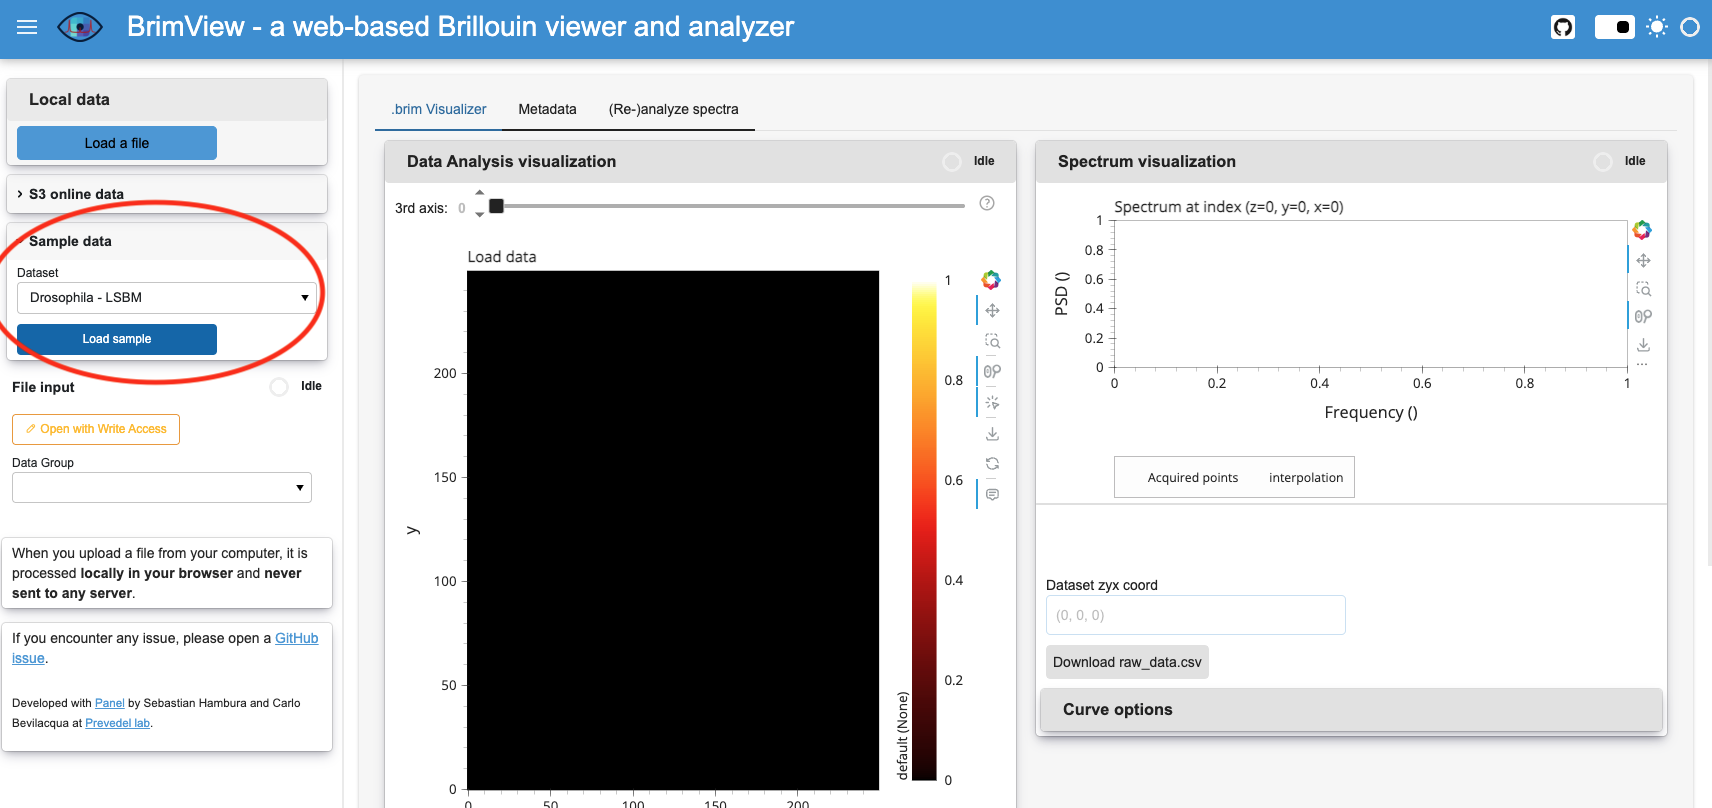
\includegraphics[width=\textwidth]{img/brimview-load_sample_data.png}
    \caption{BrimView GUI. The widget to load sample data is encircled in red.}
    \label{fig:brimview-sampledata}
\end{figure}

\subsection{Exploring the data}

Once the image is loaded you can click on any pixel and the corresponding spectrum will show on the right, including a table with the numerical values of the fitted parameters below (figure \ref{fig:brimview-spectrum}).

\begin{figure}[H]
    \centering
    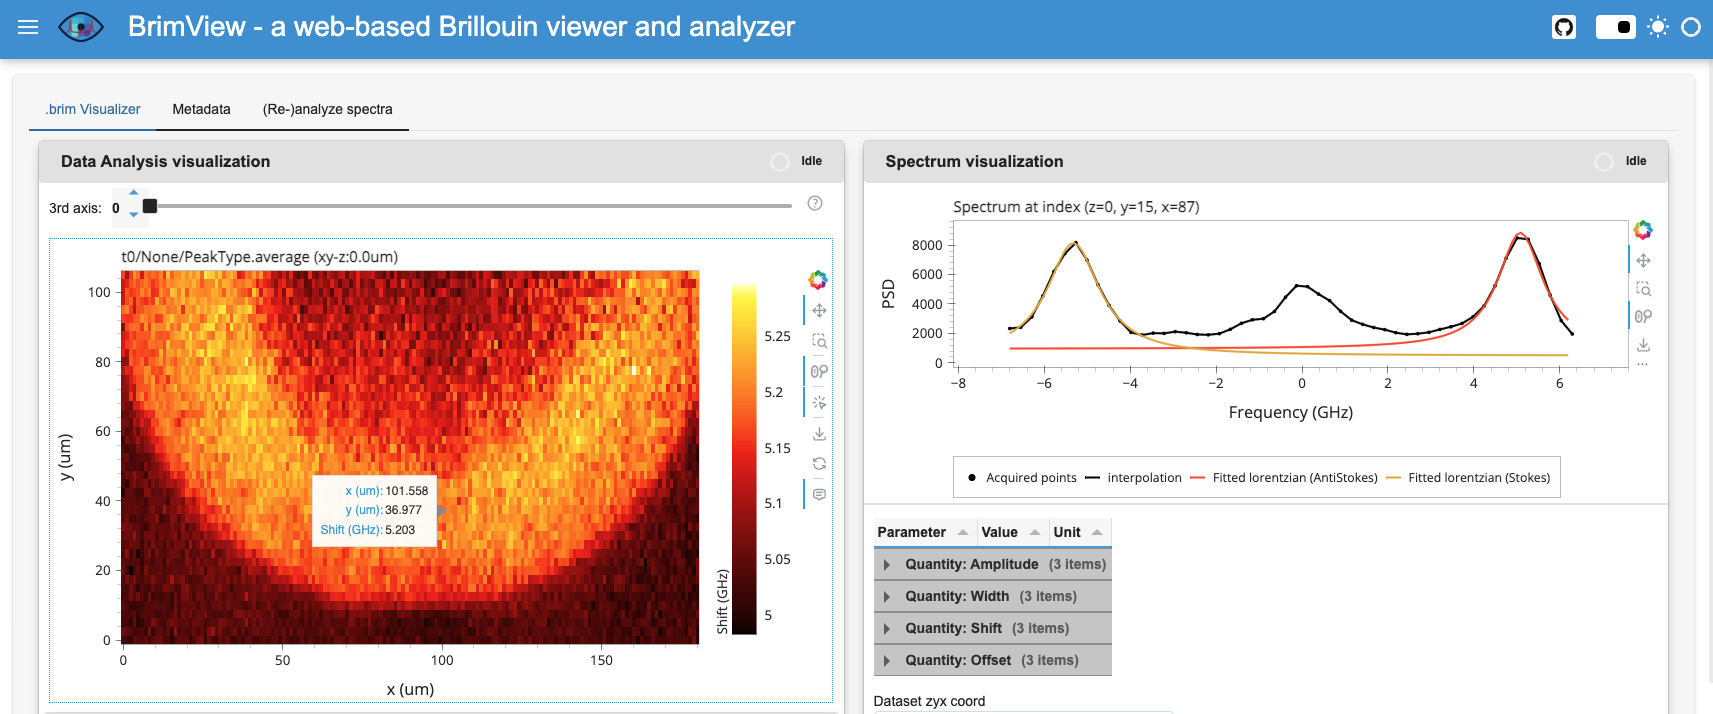
\includegraphics[width=\textwidth]{img/brimview-spectrum.png}
    \caption{The spectrum and the corresponding fitted parameters can be displayed for each pixel in the image.}
    \label{fig:brimview-spectrum}
\end{figure}

You can select which quantity (i.e. shift, linewidth, amplitude, ...), peak (i.e. Stokes, anti-Stokes, average), axis (x, y,z) and color range from the widgets below the image (figure \ref{fig:brimview-parameters}).

\begin{figure}[H]
    \centering
    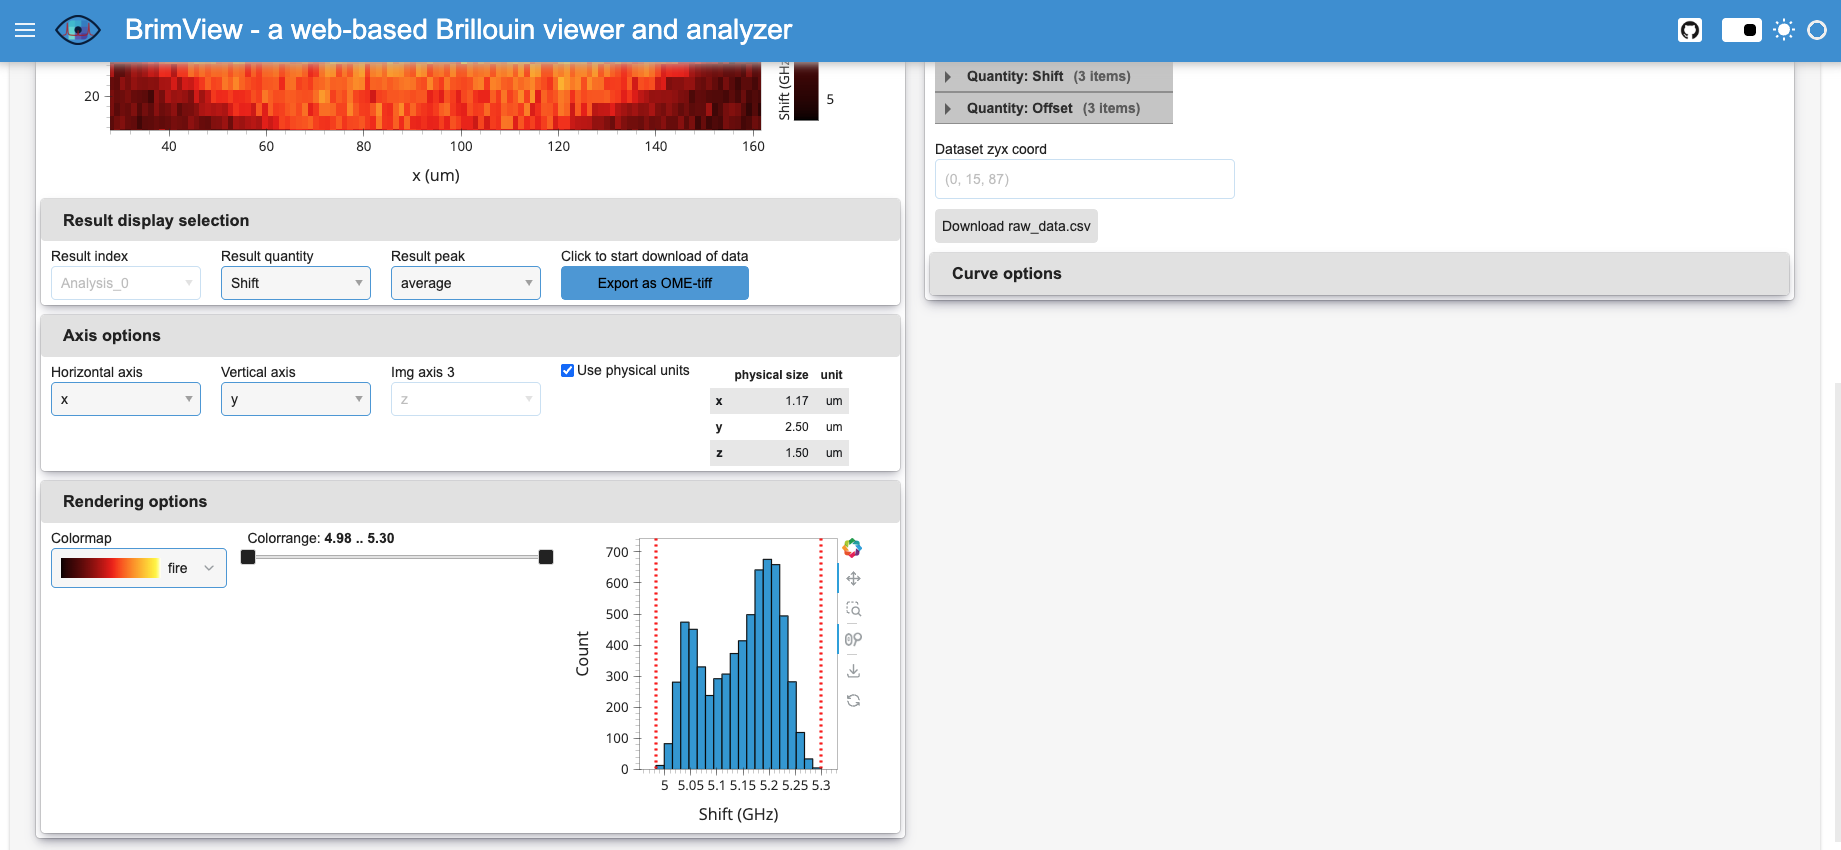
\includegraphics[width=\textwidth]{img/brimview-parameters.png}
    \caption{Different settings for displaying the image can be selected from the widgets below the images.}
    \label{fig:brimview-parameters}
\end{figure}

\section{Brimfile}

\subsection{The brim file format}

We defined a new file format - brimfile (= Brillouin imaging) - with the intent of associating spatial maps to their corresponding spectral information and metadata in a well-defined yet general and flexible fashion. More information about the brimfile format can be found \href{https://github.com/prevedel-lab/Brillouin-standard-file}{here}.

\subsection{The brimfile Python package}

To easily save data to the brim file format or read from it, we developed a Python library called \href{https://pypi.org/project/brimfile/}{brimfile}. The full documentation of the library can be found at https://prevedel-lab.github.io/brimfile/brimfile.html.

\subsubsection{Installing brimfile}
We recommend installing brimfile in a \href{https://docs.python.org/3/library/venv.html}{virtual environment}.

After activating the new environment, simply run:
\begin{lstlisting}
pip install brimfile
\end{lstlisting}
If you also need the support for exporting the analyzed data to OME-Tiff files, you can install the optional dependencies with:
\begin{lstlisting}
pip install "brimfile[export-tiff]"
\end{lstlisting}

\subsubsection{Writing to a brimfile}

Let's first of all create a function that generate sample data:
\begin{lstlisting}
import numpy as np

def generate_data():
    def lorentzian(x, x0, w):
        return 1/(1+((x-x0)/(w/2))**2)
    Nx, Ny, Nz = (7, 5, 3) # Number of points in x,y,z
    dx, dy, dz = (0.4, 0.5, 2) # Stepsizes (in um)
    n_points = Nx*Ny*Nz  # total number of points

    width_GHz = 0.4
    width_GHz_arr = np.full((Nz, Ny, Nx), width_GHz)
    shift_GHz_arr = np.empty((Nz, Ny, Nx))
    freq_GHz = np.linspace(6, 9, 151)  # 151 frequency points
    PSD = np.empty((Nz, Ny, Nx, len(freq_GHz)))
    for i in range(Nz):
        for j in range(Ny):
            for k in range(Nx):
                index = k + Nx*j + Ny*Nx*i
                #let's increase the shift linearly to have a readout 
                shift_GHz = freq_GHz[0] + (freq_GHz[-1]-freq_GHz[0]) * index/n_points
                spectrum = lorentzian(freq_GHz, shift_GHz, width_GHz)
                shift_GHz_arr[i,j,k] = shift_GHz 
                PSD[i, j, k,:] = spectrum

    return PSD, freq_GHz, (dz,dy,dx), shift_GHz_arr, width_GHz_arr
\end{lstlisting}

We can create a brimfile by doing: 
\begin{lstlisting}
from brimfile import File, Data, Metadata, StoreType
from datetime import datetime

filename = 'path/to/your/file.brim.zip' 

f = File.create(filename, store_type=StoreType.AUTO)
\end{lstlisting}
We can then add the spectral data:
\begin{lstlisting}
PSD, freq_GHz, (dz,dy,dx), shift_GHz, width_GHz = generate_data()

d0 = f.create_data_group(PSD, freq_GHz, (dz,dy,dx), name='test1')
\end{lstlisting}
and the metadata:
\begin{lstlisting}
Attr = Metadata.Item
datetime_now = datetime.now().isoformat()
temp = Attr(22.0, 'C')
md = d0.get_metadata()

md.add(Metadata.Type.Experiment, {'Datetime':datetime_now, 'Temperature':temp})
md.add(Metadata.Type.Optics, {'Wavelength':Attr(660, 'nm')})
# Add some metadata to the local data group   
temp = Attr(37.0, 'C')
md.add(Metadata.Type.Experiment, {'Temperature':temp}, local=True)
\end{lstlisting}
We can also add the result of the fit:
\begin{lstlisting}
ar = d0.create_analysis_results_group({'shift':shift_GHz, 'shift_units': 'GHz',
                                             'width': width_GHz, 'width_units': 'Hz'},
                                             {'shift':shift_GHz, 'shift_units': 'GHz',
                                             'width': width_GHz, 'width_units': 'Hz'},
                                             name = 'test1_analysis')
\end{lstlisting}
We can finally close the file:
\begin{lstlisting}
f.close()
\end{lstlisting}

\subsubsection{Reading a brimfile}
Reading from a brimfile follows a very similar logic as writing.

We first open the file:
\begin{lstlisting}
from brimfile import File, Data, Metadata

filename = 'path/to/your/file.brim.zip' 

f = File(filename)
\end{lstlisting}
We can list all the data group in the file and open the first one:
\begin{lstlisting}
#list all the data groups in the file
data_groups = f.list_data_groups(retrieve_custom_name=True)

# get the first data group in the file
d = f.get_data()
\end{lstlisting}

We can read the metadata:
\begin{lstlisting}
# get the metadata 
md = d.get_metadata()
all_metadata = md.all_to_dict()
# the list of metadata is defined here https://github.com/prevedel-lab/Brillouin-standard-file/blob/main/docs/brim_file_metadata.md
time = md['Experiment.Datetime']
time.value
time.units
temp = md['Experiment.Temperature']
md_dict = md.to_dict(Metadata.Type.Experiment)
\end{lstlisting}

We can get the results of the analysis:
\begin{lstlisting}
#get the list of analysis results in the data group
ar_list = d.list_AnalysisResults(retrieve_custom_name=True)
# get the first analysis results in the data group
ar = d.get_analysis_results()
\end{lstlisting}
and the corresponding image: 
\begin{lstlisting}
# get the image of the shift quantity for the average of the Stokes and anti-Stokes peaks
img, px_size = ar.get_image(Data.AnalysisResults.Quantity.Shift, Data.AnalysisResults.PeakType.average)
# get the units of the shift quantity
u = ar.get_units(Data.AnalysisResults.Quantity.Shift)
\end{lstlisting}
We can save the image as a TIFF: 
\begin{lstlisting}
ar_cls = Data.AnalysisResults
ar.save_image_to_OMETiff(ar_cls.Quantity.Shift, ar_cls.PeakType.average, filename='path/to/your/exported_tiff' )
\end{lstlisting}
We can also get the spectrum corresponding to a specific pixel:
\begin{lstlisting}
coord = (1,3,4)
PSD, frequency, PSD_units, frequency_units = d.get_spectrum_in_image(coord)
\end{lstlisting}

We can finally close the file:
\begin{lstlisting}
f.close()
\end{lstlisting}

\section{HDF5\_BLS package}

The HDF5\_BLS package is a Python package for creating BrimX files, a file format based on HDF5, designed to support all Brillouin-related data in a human-readable way, and be integrated to all existing workflows of the community. It is compatible with Python 3.10 and above. 

\subsection{Installation}

We recommend setting up a virtual environment to install the package. This can be done using the following command:

\begin{tcolorbox}[colback=blue!5, colframe=blue!40!black, boxrule=0.5mm, sharp corners, left=2mm, right=2mm, top=1mm, bottom=1mm]
- On Mac terminal
\begin{lstlisting}
python -m venv HDF5_BLS_venv
source HDF5_BLS_venv/bin/activate 
\end{lstlisting}
\end{tcolorbox}

\begin{tcolorbox}[colback=yellow!5, colframe=yellow!40!black, boxrule=0.5mm, sharp corners, left=2mm, right=2mm, top=1mm, bottom=1mm]
- On Windows terminal
\begin{lstlisting}
python -m venv HDF5_BLS_venv
HDF5_BLS_venv\Scripts\activate
\end{lstlisting}
\end{tcolorbox}

On both OS, the package can be installed using pip:
\begin{lstlisting}
pip install HDF5_BLS
\end{lstlisting}


\subsection{An example}

Here we propose to create a synthetic Brillouin dataset that we'll store in a BrimX file. We will store 3 different types of synthetic data:
\begin{itemize}
    \item A single spectrum 
    \item A synthetic time evolution
    \item A spatial mapping in 2D
    \item A z-stack of a sphere
\end{itemize}

\subsubsection{Creating the data}

Let's define a general DHO function to create the Brillouin spectra.

\begin{lstlisting}
def DHO(nu, nu0, gamma, a, b):
    return b + a * (gamma*nu0)**2/((nu**2-nu0**2)**2+(gamma*nu)**2)
\end{lstlisting}

Let's now define a frequency axis to create the spectra.

\begin{lstlisting}
nu = np.linspace(-15, 15, 1024)
\end{lstlisting}

Let's now build synthetic datasets to image different scenarios:
\begin{itemize}
    \item 0D: Let's say we have a single spectrum, with a Brillouin shift of 5 GHz and linewidth of 1 GHz. Let's give the spectrum an amplitude of 1 and no offset.
\begin{lstlisting}
shift_0D = 5
linewidth_0D = 1
PSD_0D = DHO(nu, shift_0D, linewidth_0D, 1, 0)
\end{lstlisting}
    \item 1D: Let's do the same for a 1D dataset now, let's think about a simple time evolution of a sample, where the shift rises quadratically from 5 to 6 GHz over time, and the linewidth from 1 to 2 GHz linearly. Here again, let's keep an amplitude of 1 with no offset.
\begin{lstlisting}
time_1D = np.linspace(0, 10, 100)
shift_1D = 5 + time**2/100
linewidth_1D = np.linspace(1, 2, 100)
for s, l in zip(shift_1D, linewidth_1D):
    PSD_1D = DHO(nu, s, l, 1, 0)
\end{lstlisting}
    \item 2D: Let's consider a mapping showing a diagonal shift gradient from 5 to 6 GHz, and a diagonal linewidth gradient from 1 to 2 GHz. We keep an amplitude of 1 with no offset.
\begin{lstlisting}
gradient_x = np.linspace(0, 1, 50)
gradient_y = np.linspace(0, 1, 50)
temp = (np.outer(gradient_y, gradient_x) + np.outer(gradient_y, gradient_x))/2
shift_2D = temp + 5
linewidth_2D = temp + 1 
PSD_2D = np.zeros((50, 50, 1024))
for i in range(50):
    for j in range(50):
        PSD_2D[i, j] = DHO(nu, shift_2D[i, j], linewidth_2D[i, j], 1, 0) 
\end{lstlisting}
    \item 3D: Let's now think about a z-stack. In this example we'll do a z-stack of a sphere embedded in a solution. The solution will have a shift of 5GHz and linewidth 1GHz, while the sphere will have a shift of 6GHz and linewidth 2GHz. Again, we'll keep an amplitude of 1 with no offset. Again, we have an amplitude of 1 and an offset of 0 for all spectra.
\begin{lstlisting}
x = np.linspace(-1, 1, 50)
y = np.linspace(-1, 1, 50)
z = np.linspace(-1, 1, 50)
shift_3D = np.zeros((50, 50, 50))
linewidth_3D = np.zeros((50, 50, 50))
PSD_3D = np.zeros((50, 50, 50, 1024))
for i in range(50):
    for j in range(50):
        for k in range(50):
            if (x[i]**2 + y[j]**2 + z[k]**2) > 1:
                shift_3D[i, j, k] = 5 
                linewidth_3D[i, j, k] = 1 
            else:
                shift_3D[i, j, k] = 6 
                linewidth_3D[i, j, k] = 2 
            PSD_3D[i, j, k] = DHO(nu, shift_3D[i, j, k], linewidth_3D[i, j, k], 1, 0)
\end{lstlisting}
\end{itemize}

You can of course look at the PSD, shift and linewidth arrays with your favorite visualization tools (e.g. matplotlib).

\subsubsection{Adding the data to a BrimX file}

Here we're going to structure our file to store the four different datasets we've created. Each dataset will be stored in a separate group that we'll name with example names.

First we create the BrimX file at a given path, and define an object "wrp" to interact with it.
\begin{lstlisting}
wrp = wrapper.Wrapper('path/to/file.h5')
\end{lstlisting}

For this example, we will structure the file as follows:
\begin{verbatim}
file.h5
|- Brillouin
|  |- A single spectrum 
|  |- A time series
|  |- A mapping
|  |- A z-stack
\end{verbatim}

In each of these groups, we'll store the corresponding Power spectral density datasets, frequency array and shift and linewidth arrays. To do so, we will use the three following functions:
\begin{itemize}
    \item "add\_frequency": to store the frequency array
    \item "add\_PSD": to store the Power spectral density array
    \item "add\_treated\_data": to store the shift and linewidth arrays
\end{itemize}
Each of these functions work the same way:
\begin{enumerate}
    \item You indicate the dataset to add.
    \item You specify where the dataset will be stored in the file (argument "parent\_group").
    \item You provide a name for the dataset (argument "name").
\end{enumerate}

Because you might need in the future to add other treatment modalities, we have made it so that all the datasets obtained after treatment are added in a same group. Therefore instead of "name" the "add\_treated\_data" function takes "name\_group" as argument, which is the name of the group where all the treated datasets will be stored. The names of the datasets themselves will be the type of data by default (e.g. "Shift" for the shift array, "Linewidth" for the linewidth array, etc.).

With the provided code, this gives us:

\begin{lstlisting}
# Adding the 0D datasets
wrp.add_frequency(data=nu, parent_group="Brillouin/A single spectrum", name = "Frequency")
wrp.add_PSD(data=PSD_0D, parent_group="Brillouin/A single spectrum", name = "PSD")
wrp.add_treated_data(parent_group="Brillouin/A single spectrum", name_group = "Treated Data", shift = shift_0D, linewidth = linewidth_0D)

# Adding the 1D datasets
wrp.add_frequency(data=nu, parent_group="Brillouin/A time series", name = "Frequency")
wrp.add_PSD(data=PSD_1D, parent_group="Brillouin/A time series", name = "PSD")
wrp.add_treated_data(parent_group="Brillouin/A time series", name_group = "Treated Data", shift = shift_1D, linewidth = linewidth_1D)

# Adding the 2D datasets
wrp.add_frequency(data=nu, parent_group="Brillouin/A mapping", name = "Frequency")
wrp.add_PSD(data=PSD_2D, parent_group="Brillouin/A mapping", name = "PSD")
wrp.add_treated_data(parent_group="Brillouin/A mapping", name_group = "Treated Data", shift = shift_2D, linewidth = linewidth_2D)

# Adding the 3D datasets
wrp.add_frequency(data=nu, parent_group="Brillouin/A z-stack", name = "Frequency")
wrp.add_PSD(data=PSD_3D, parent_group="Brillouin/A z-stack", name = "PSD")
wrp.add_treated_data(parent_group="Brillouin/A z-stack", name_group = "Treated Data", shift = shift_3D, linewidth = linewidth_3D)
\end{lstlisting}

You are now the proud owner of a BrimX file containing synthetic Brillouin datasets!

Note: you can add other types of datasets to the BrimX file. The available types are:

\begin{itemize}
    \item "Frequency" with the function "add\_frequency"
    \item "PSD" with the function "add\_PSD"
    \item "Other" with the function "add\_other", this can be anything you want to store (grayscale images, Raman spectra, fluorescence maps...)
    \item "Raw Data" with the function "add\_raw\_data", where you can store your data "as is" (what the spectrometer returns).
    \item "Abscissa" with the function "add\_abscissa" to add abscissa for your axis. Please refer to footnote \cprotect\footnote{In that case, you need to provide, aside from the dataset itself, the place where to store it and its name, the units of the abscissa (attribute "unit" given as a string, for example "mm" or "K"), the first dimension of the PSD it applies to and the last dimension of the PSD it applies to (attributes "dim\_strart" and "dim\_end" respectively, given as integers and with the usual convention: starting from 0, starting index included, ending index excluded). For example:
\begin{lstlisting}
    t = np.linspace(0,10,100) # 100 values of time ranging from 0 to 10s
    PSD = np.random.random((100,512)) # 100 PSD associated to the time array
    wrp.add_PSD(data = PSD, parent_group = "Brillouin/A new time series", name = "PSD")
    wrp.add_abscissa(data = t, parent_group = "Brillouin/A new time series", name = "Time", unit = "s", dim_start = 0, dim_end = 1)
\end{lstlisting}}
\end{itemize}

You can also add other types of datasets after treatment, in that case you will use the "add\_treated\_data" function and just specify the datasets you want to add from this list:
\begin{itemize}
    \item A record of shift values -> argument "shift"
    \item A record of linewidth values -> argument "linewidth"
    \item A record of the values of amplitude -> argument "amplitude"
    \item Values for the loss tangent -> argument "BLT" 
    \item A record for the errors on the shift values -> argument "shift\_err"
    \item A record for the errors on the linewidth values -> argument "linewidth\_err"
    \item A record for the errors on the amplitude values -> argument "amplitude\_err"
    \item A record for the errors on the BLT values -> argument "BLT\_err"
\end{itemize}


\subsubsection{Adding metadata to the BrimX file}

To add metadata to the BrimX file, we will choose the easy way for this example, and just edit the standard spreadsheet given with the package and downloadable at this link: \url{https://github.com/bio-brillouin/HDF5_BLS/blob/main/spreadsheets/attributes_v1.0.xlsx}.

A list of established parameters is given, their name, units and definition is written in the different columns. For this example, we are filling the datasheet as presented on figure \ref{fig:excel_attributes}.
\begin{figure}[H]
    \centering
    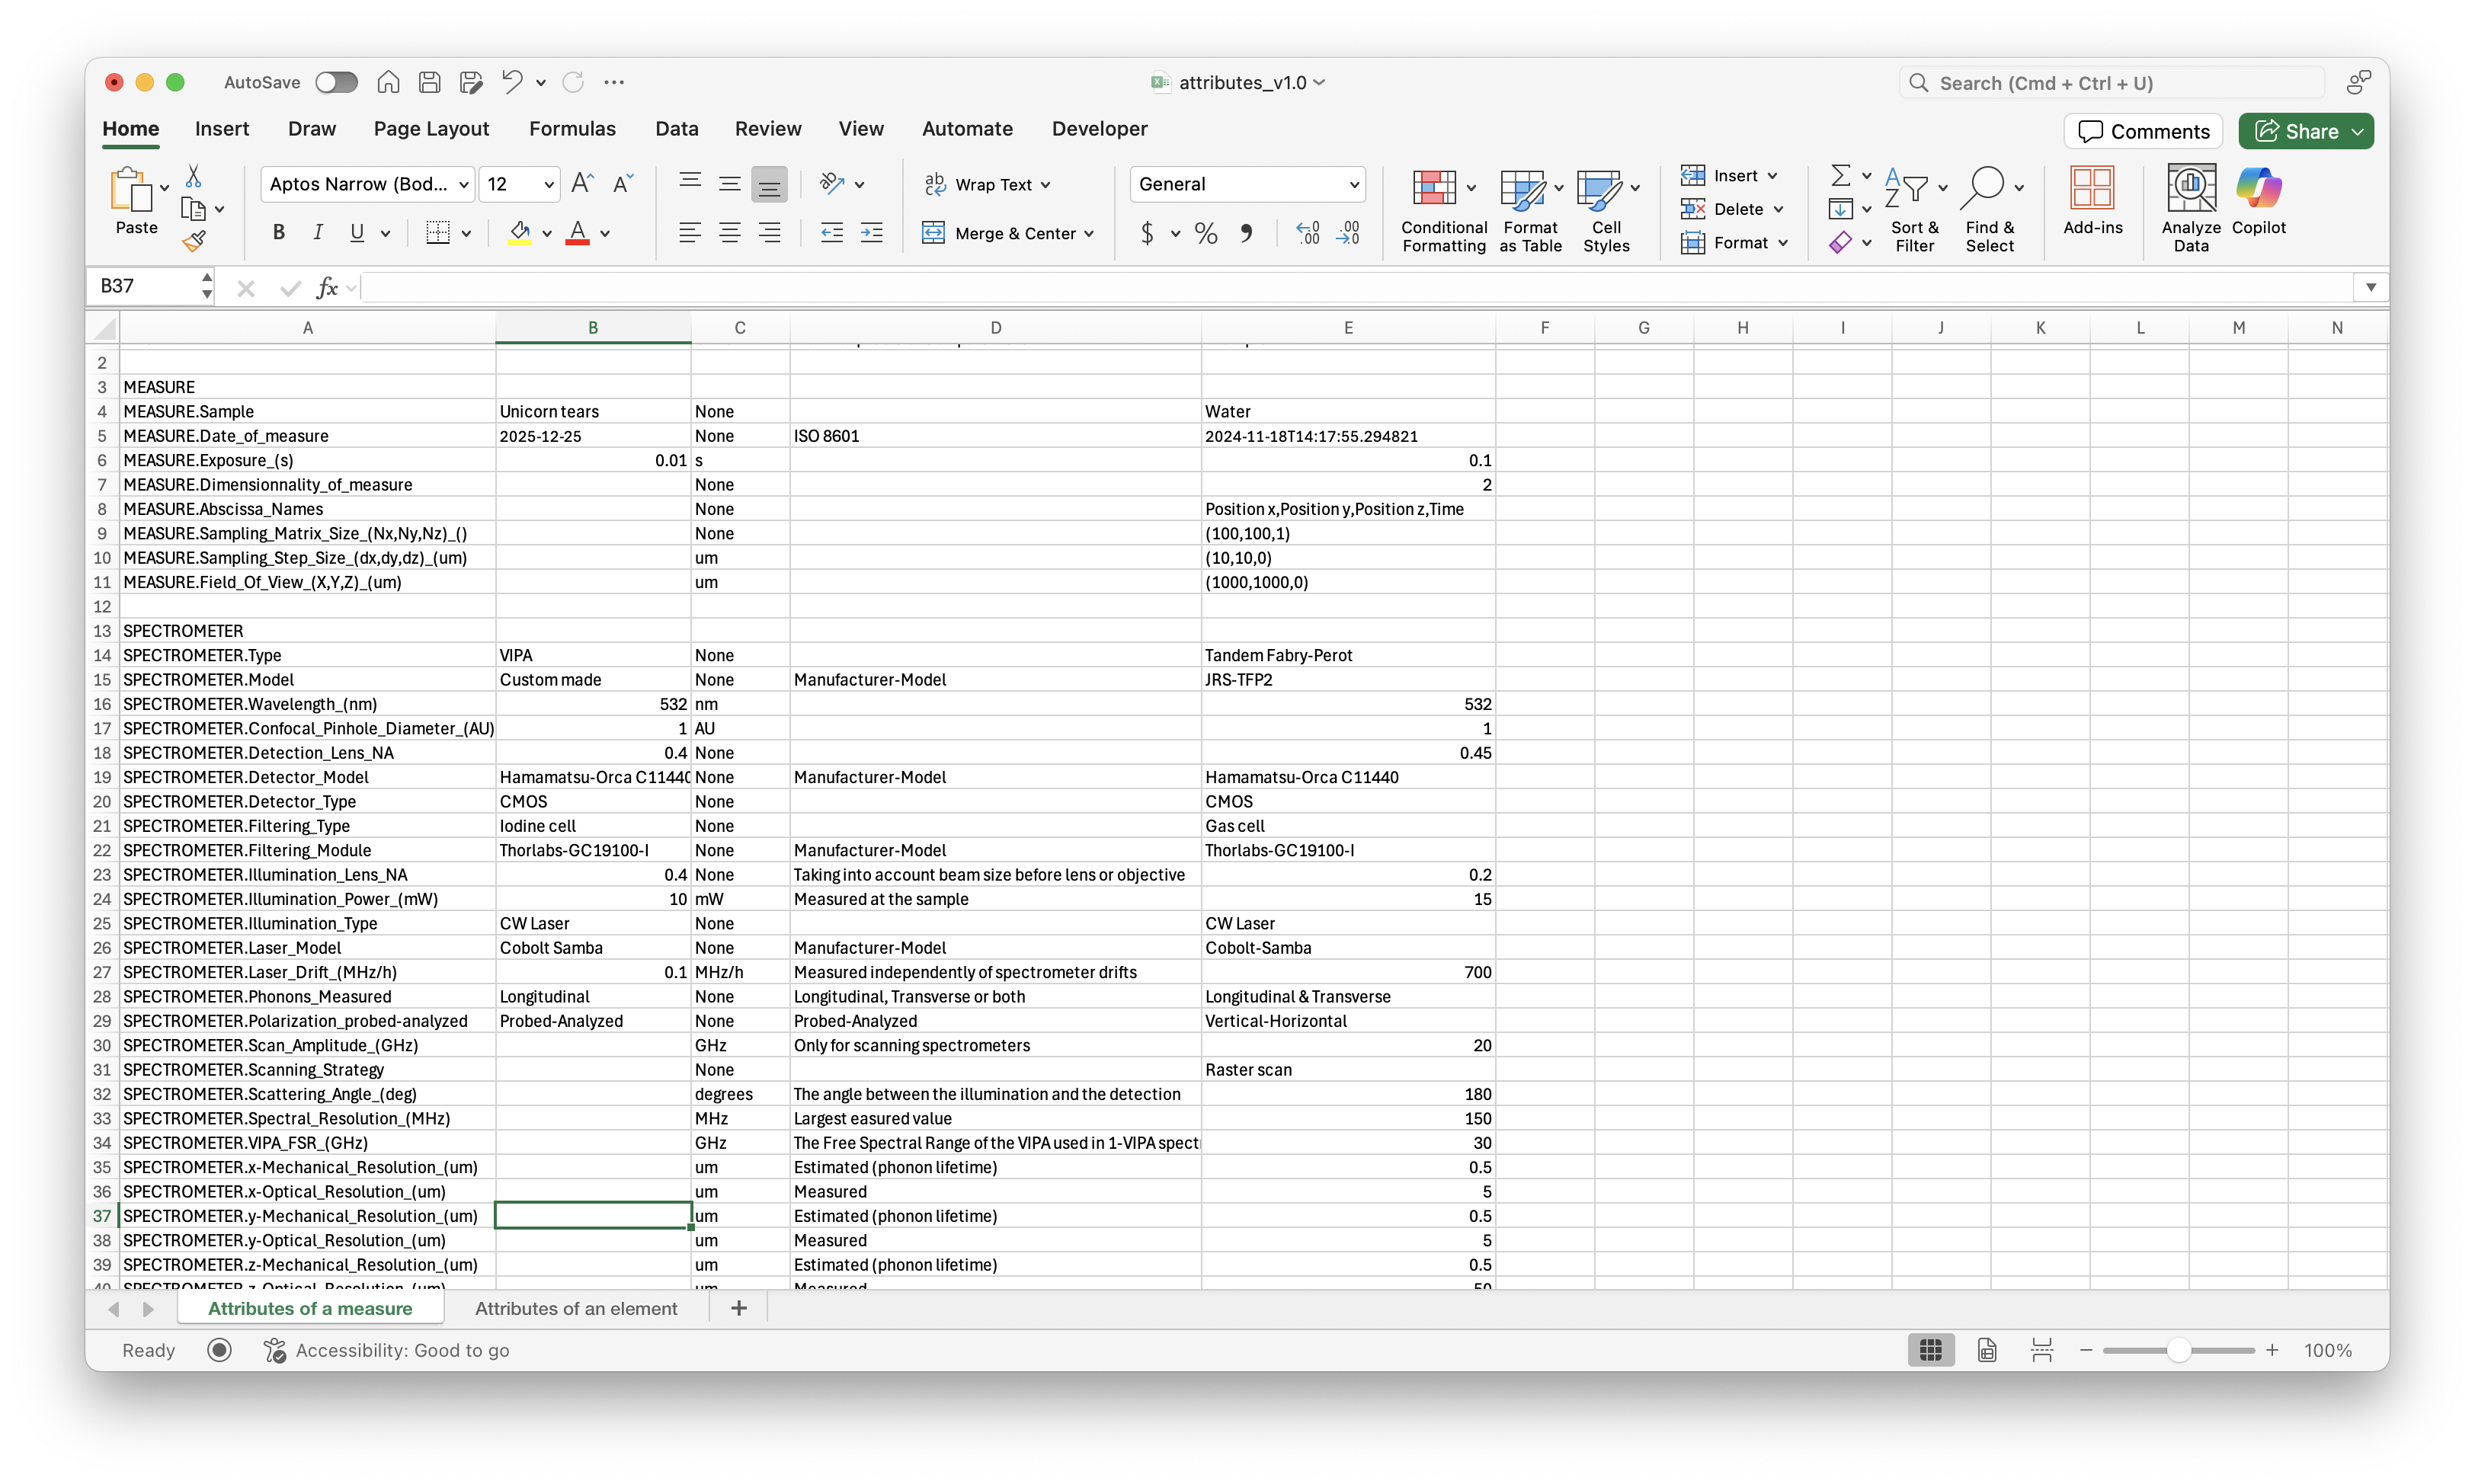
\includegraphics[width=\textwidth]{img/Excel_attributes.png}
    \caption{Example of the filled datasheet used to add metadata to the BrimX file}
    \label{fig:excel_attributes}
\end{figure}

You can of course play with this file, add your own parameters, change the values for the ones given, add values for the ones not given, etc. We recommend however not changing the names of the existing parameters so that all the community calls the same parameters the same way.

You can then save the file at your prefered location, and apply it to the BrimX file you just created. To do so, you can use the following code:

\begin{lstlisting}
wrp.import_properties_data(filepath='path/to/attributes.xlsx')
\end{lstlisting}

This line of code applies the metadata to the whole BrimX file. You can also add metadata only to a specific group by adding the argument "path" to the function:

\begin{lstlisting}
wrp.import_properties_data(filepath='path/to/attributes.xlsx', path = "Brillouin/A z-stack")
\end{lstlisting}


\subsection{Template for integrating BrimX files to your workflow}

You can now try integrating the use of BrimX files in your workflow. Note that the example we showed above is limited to 4 kinds of datasets (frequency, PSD, shift and linewidth). The format can handle a total of 13 different kinds of datasets that are defined in the documentation of the package: \url{https://github.com/bio-brillouin/HDF5_BLS/blob/main/guides/Tutorial/Tutorial.pdf}.

Here is a base template to get you started:

\begin{lstlisting}
import HDF5_BLS as bls

# Create a BrimX file
wrp = bls.Wrapper(filepath = "path/to/file.h5")

###############################################################################
# Existing code to extract data from a file
###############################################################################
# Storing the data in the HDF5 file (for this example we use a random array)
data = np.random.random((50, 50, 512))
wrp.add_raw_data(data = data, parent_group = "Brillouin", name = "Raw data")

###############################################################################
# Existing code to convert the data to a PSD
###############################################################################
# Storing the Power Spectral Density in the HDF5 file together with the associated frequency array (for this example we use random arrays)
PSD = np.random.random((50, 50, 512))
frequency = np.arange(512)
wrp.add_PSD(data = PSD, parent_group = "Brillouin", name = "Power Spectral Density")
wrp.add_frequency(data = frequency, parent_group = "Brillouin", name = "Frequency")

###############################################################################
# Existing code to fit the PSD to extract shift and linewidth arrays
###############################################################################
# Storing the Power Spectral Density in the HDF5 file together with the associated frequency array (for this example we use random arrays)
shift = np.random.random((50, 50))
linewidth = np.random.random((50, 50))
wrp.add_treated_data(parent_group = "Brillouin", name_group = "Treat_0", shift = shift, linewidth = linewidth)
\end{lstlisting}

\subsection{Extracting data from the BrimX file}

You can now interact directly with the BrimX file as any other file storing data. To extract a dataset located at a known path in the file, you can use the following line of code:
\begin{lstlisting}
dataset = wrp["path/to/dataset/in/the/file"][:]
\end{lstlisting}

For example, using the example BrimX file we created in this tutorial, you can extract the PSD of the first spectrum using the following code:
\begin{lstlisting}
psd = wrp["Brillouin/A single spectrum/PSD"][:]
\end{lstlisting}

To extract the metadata that is applied to an element of the file, you can use the following code:
\begin{lstlisting}
metadata = wrp.get_attributes("Brillouin/A single spectrum/PSD")
\end{lstlisting}
This will list all the metadata applied to the dataset located at the given path (in that case the PSD of the single spectrum).

The paths can be obtained by visualizing the file as explained in the next section.

\subsection{Visualizing the BrimX file}

\subsubsection{Online}

You can visualize the BrimX file online using the myhdf5 web application: \url{https://myhdf5.hdfgroup.org}. This application runs locally in your web browser so you can use it safely even to observe sensitive data.

When you open the application, you can upload your BrimX file and explore its contents either by clicking the "Select HDF5 File" button or by dragging and dropping your file in the window (figure \ref{fig:my_hdf5_welcome}). Let's try with the example file we created in this tutorial.

\begin{figure}[H]
    \centering
    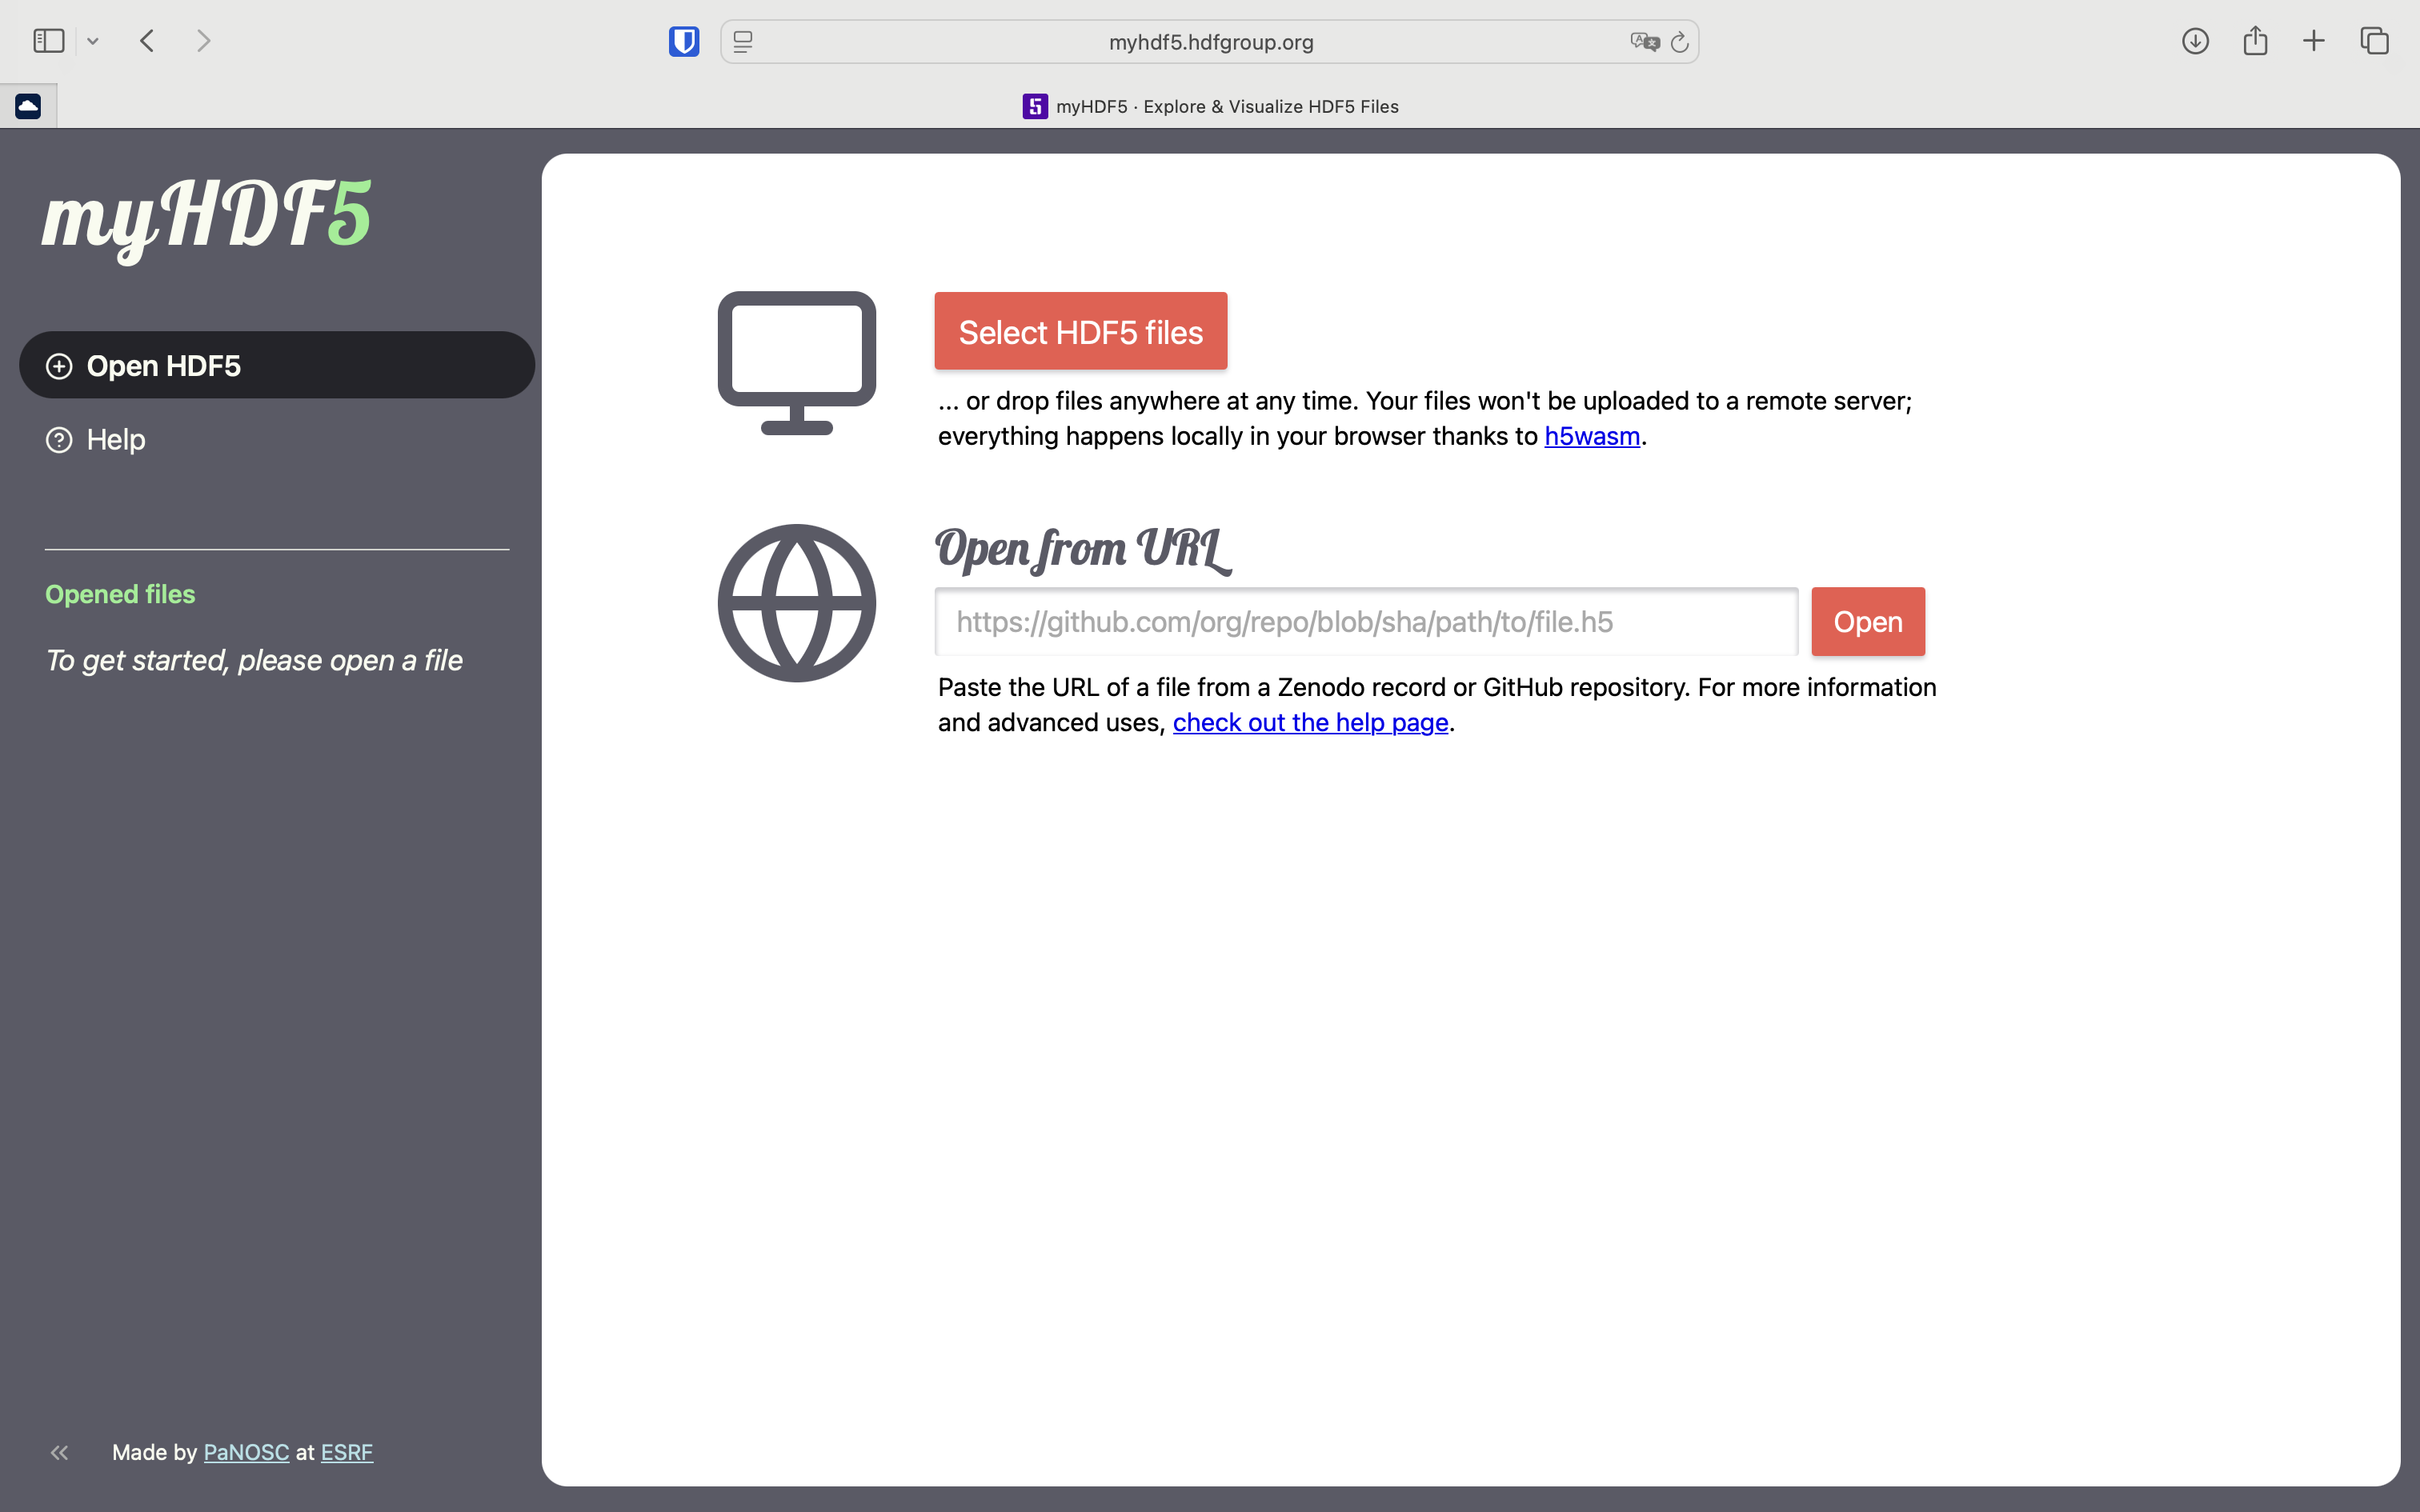
\includegraphics[width=0.8\textwidth]{img/MyHDF5_welcome_window.png}
    \caption{The welcome window of the myhdf5 application}
    \label{fig:my_hdf5_welcome}
\end{figure}

Once your file is loaded, you can explore its contents on the left panel (figure \ref{fig:my_hdf5_structure}).

\begin{figure}[H]
    \centering
    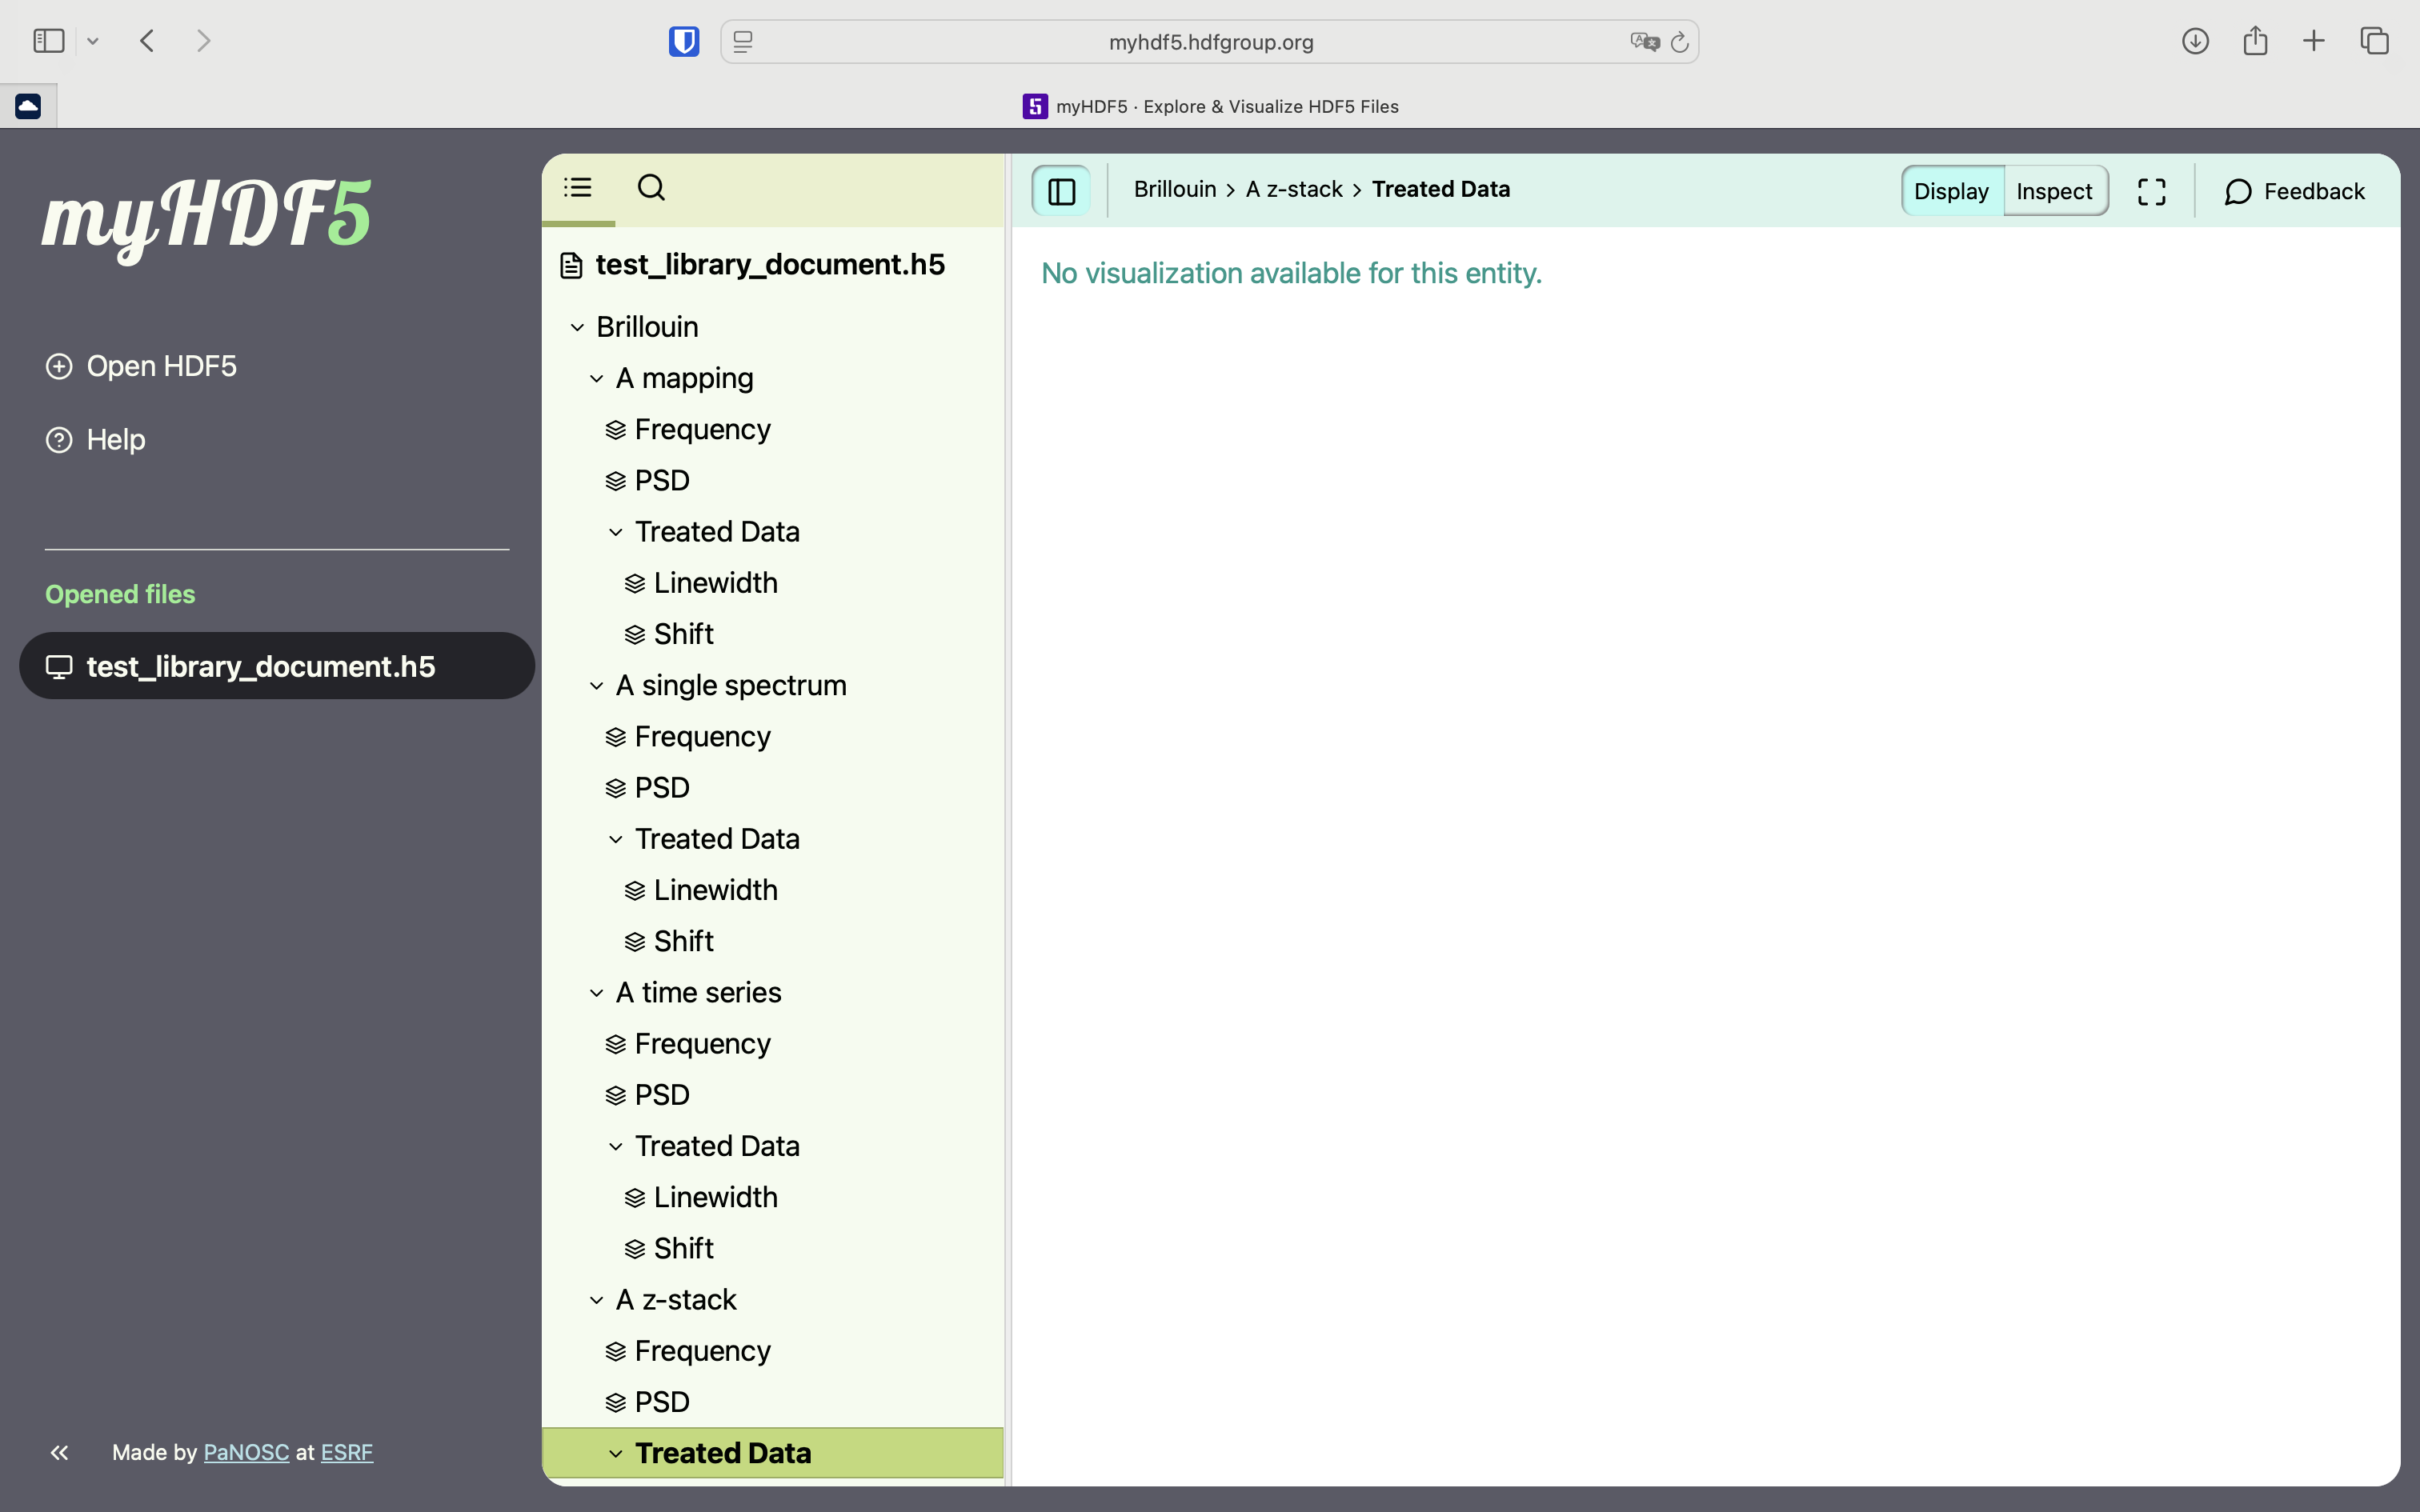
\includegraphics[width=0.8\textwidth]{img/MyHDF5_Developped structure.png}
    \caption{The developed structure view of your HDF5 file in the myhdf5 application}
    \label{fig:my_hdf5_structure}
\end{figure}

From there you can explore the file, visualize attributes (figure \ref{fig:my_hdf5_attributes}) and datasets of any dimension (figure \ref{fig:my_hdf5_datasets}).

\begin{figure}[H]
    \centering
    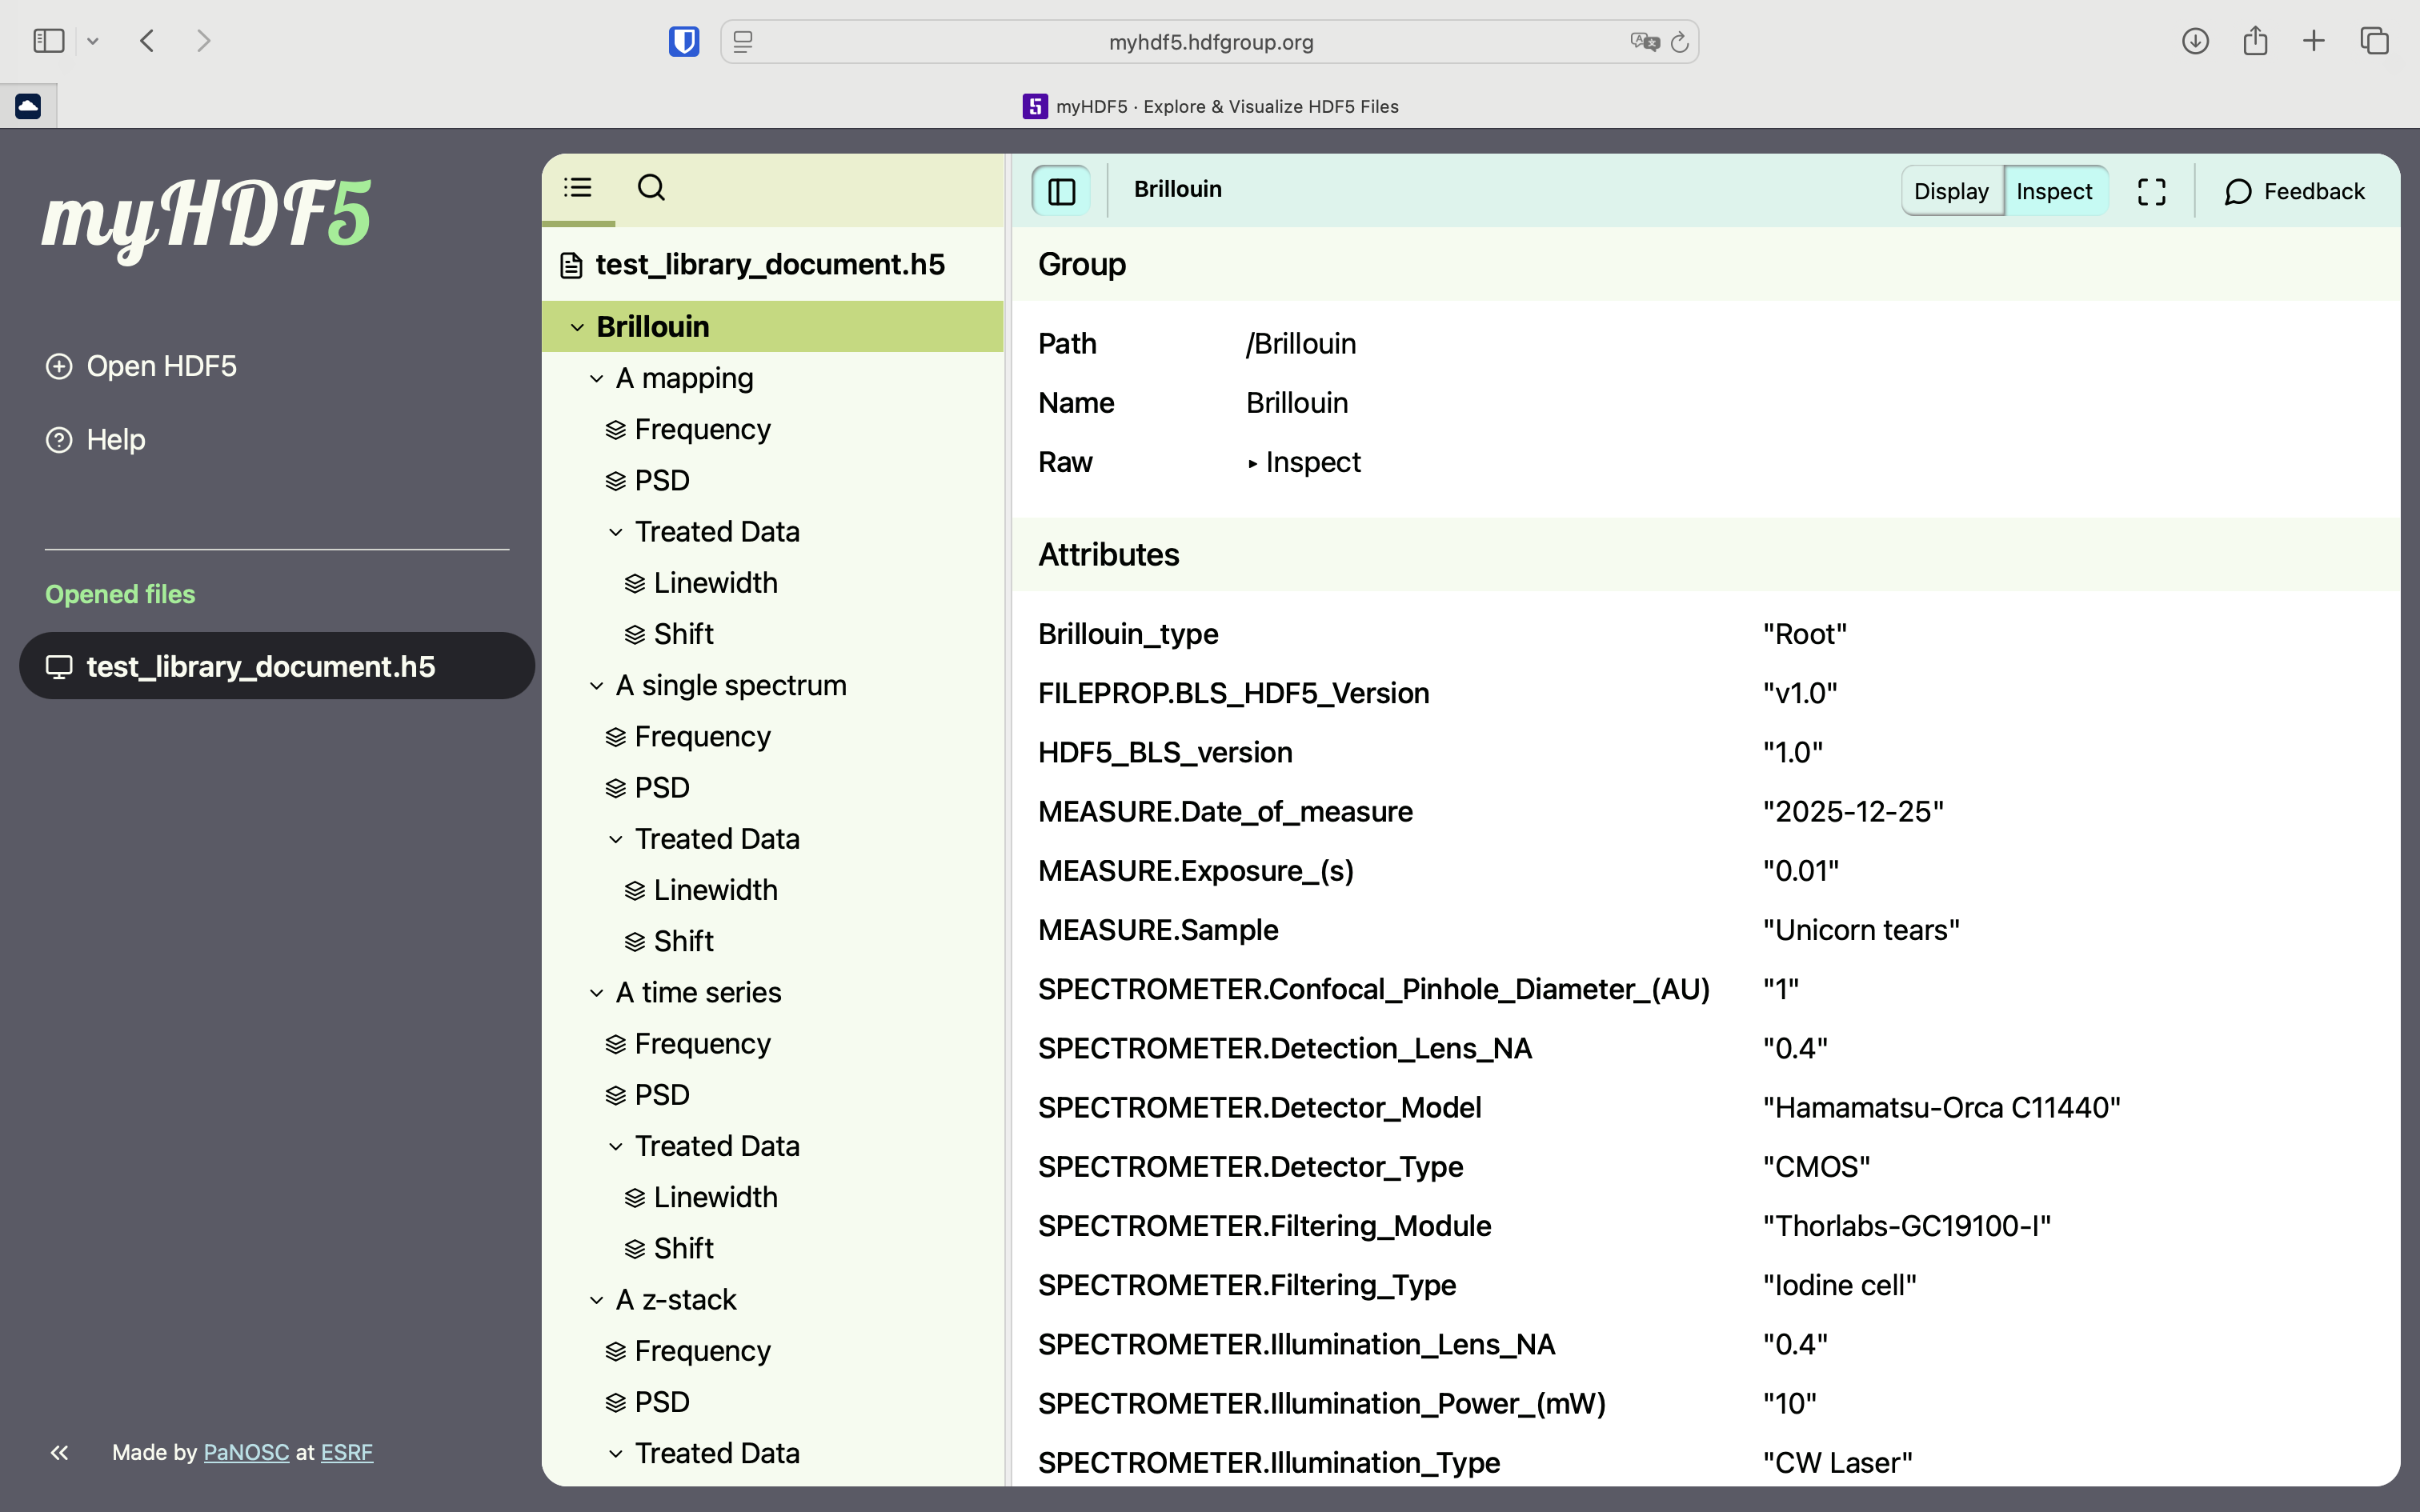
\includegraphics[width=0.8\textwidth]{img/My_HDF5_attributes.png}
    \caption{Visualizing the attributes stored in the "Brillouin" group} 
    \label{fig:my_hdf5_attributes}
\end{figure}

\begin{figure}[H]
    \centering
    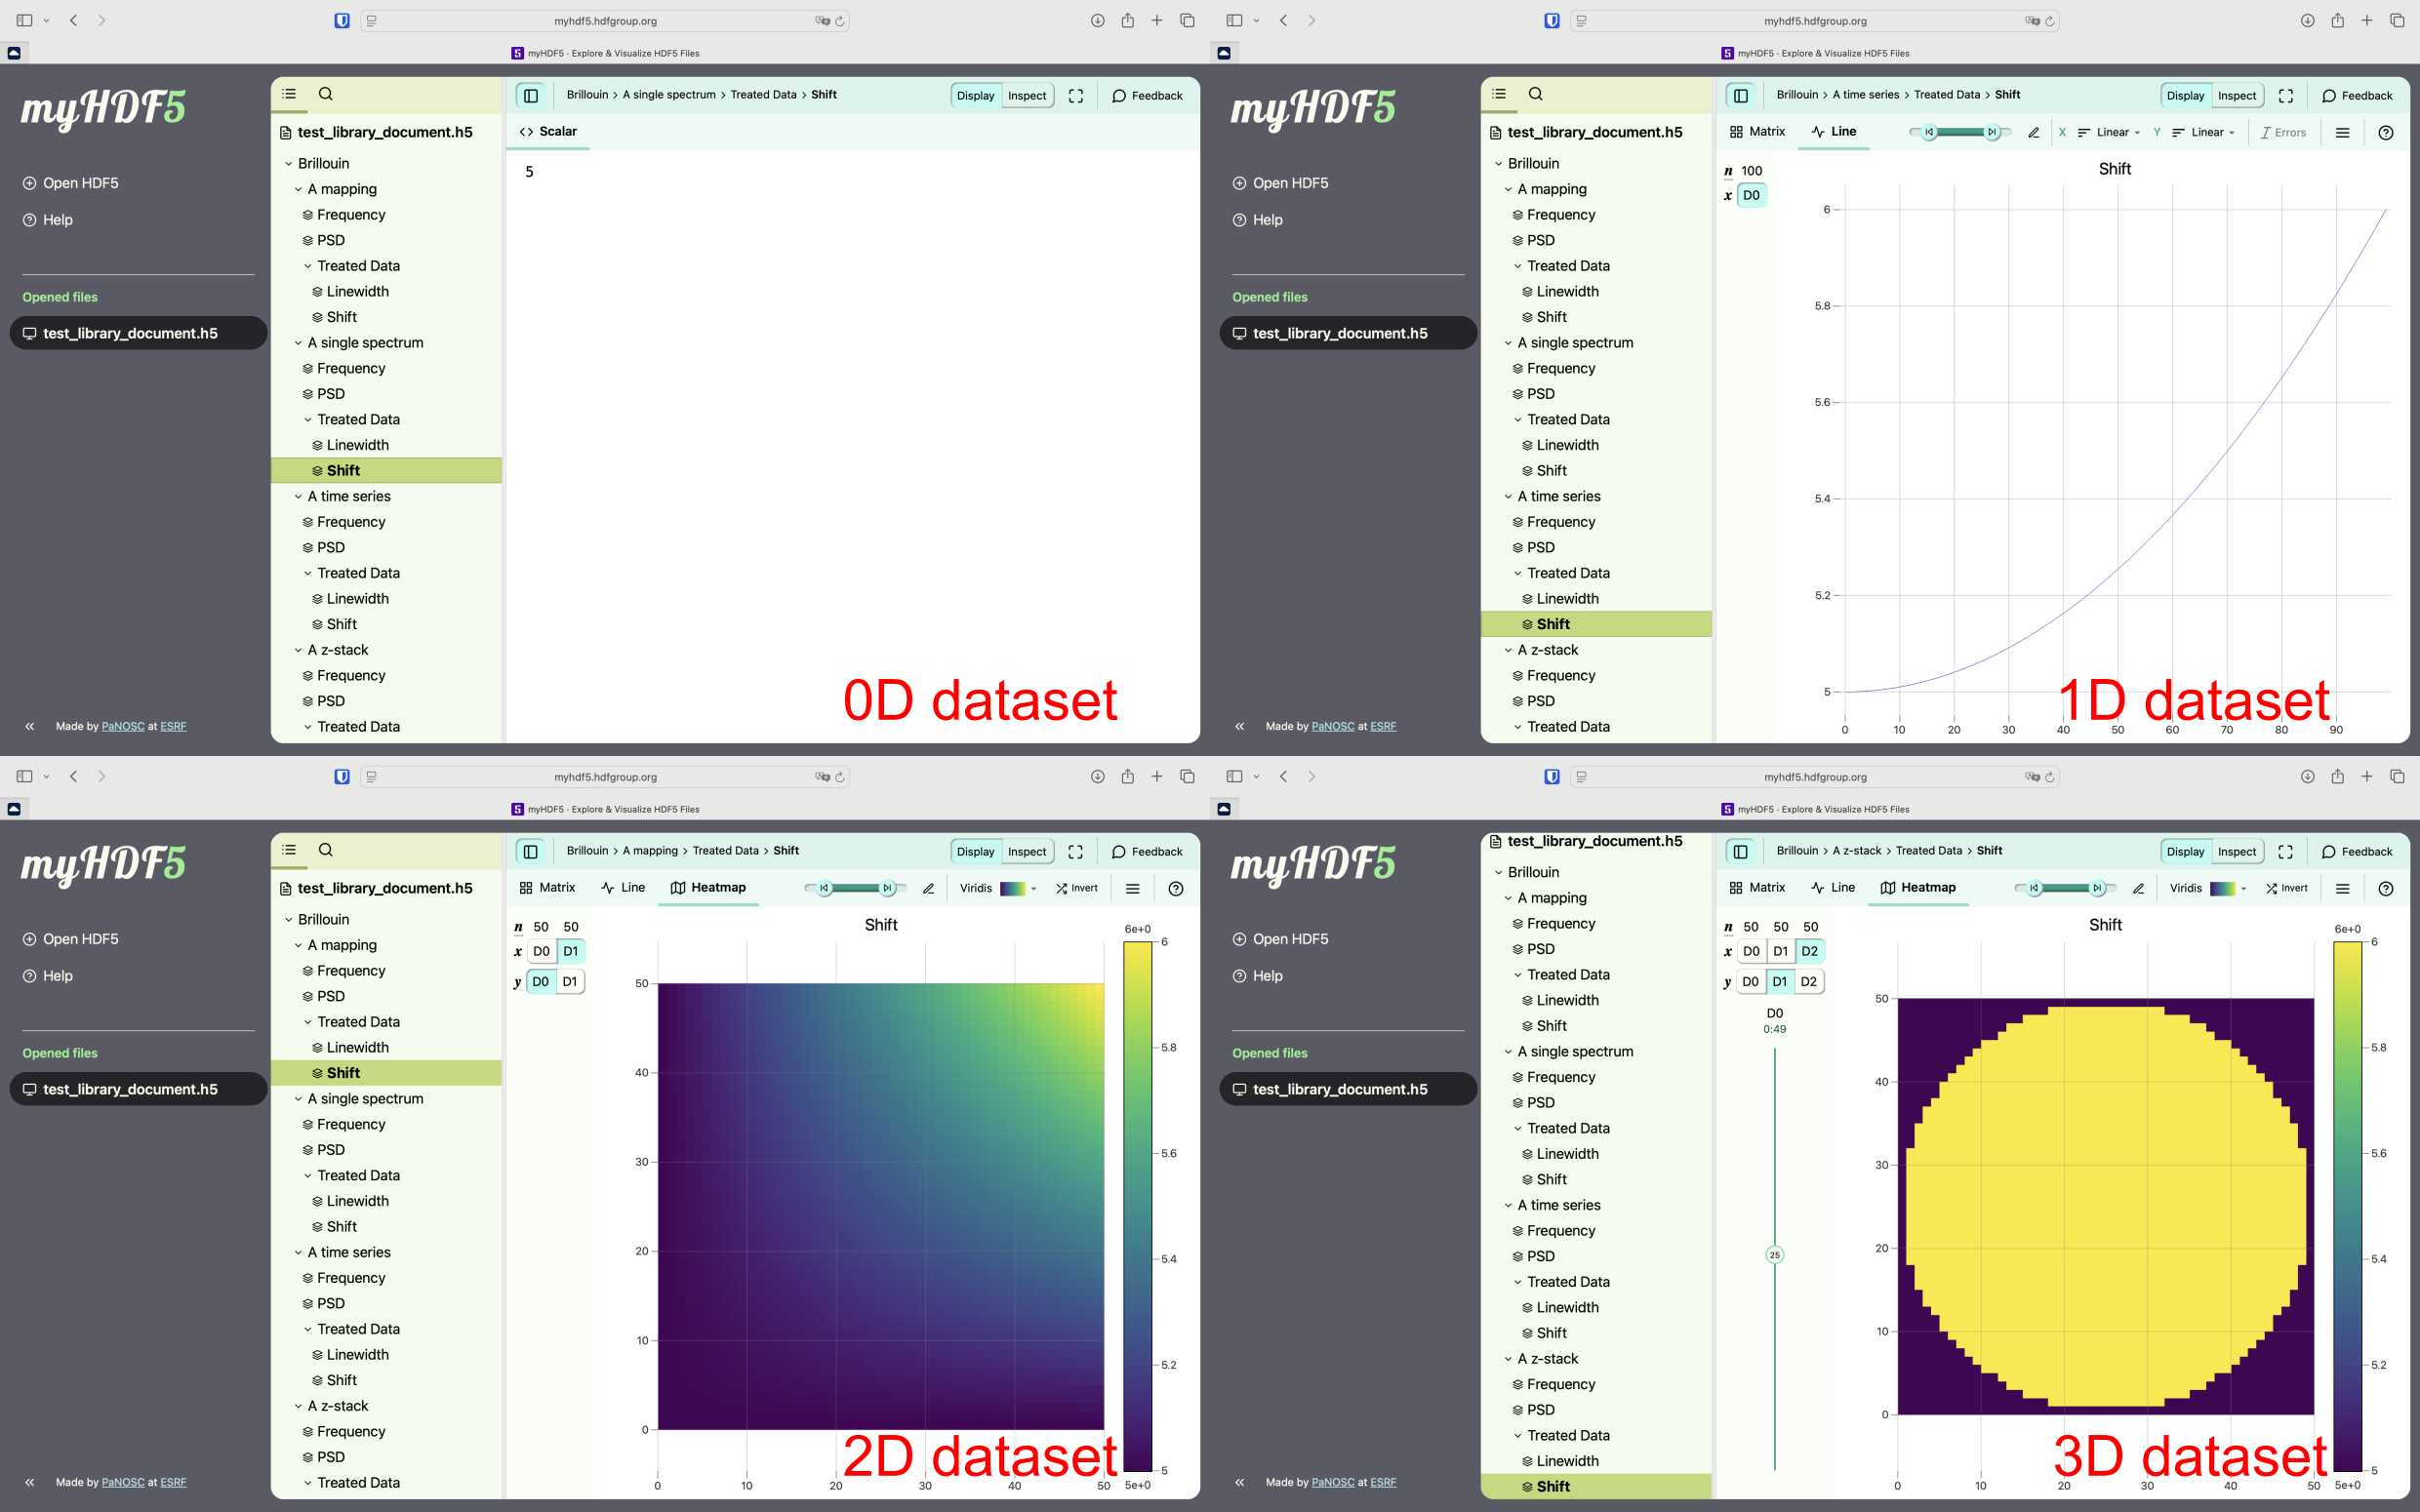
\includegraphics[width=\textwidth]{img/MyHDF5_visualizer.png}
    \caption{Visualizing the datasets using the MyHDF5 web application} 
    \label{fig:my_hdf5_datasets}
\end{figure}

\subsubsection{Using Panoply}

Panoply is an application developed by NASA to visualize geo-referenced data and more generally HDF5 files (thank you NASA!). It can be downloaded for free at this link: \url{https://www.giss.nasa.gov/tools/panoply/}. 

Here are some screenshots of the application with the example file we created in this tutorial: 

\begin{figure}[H]
    \centering
    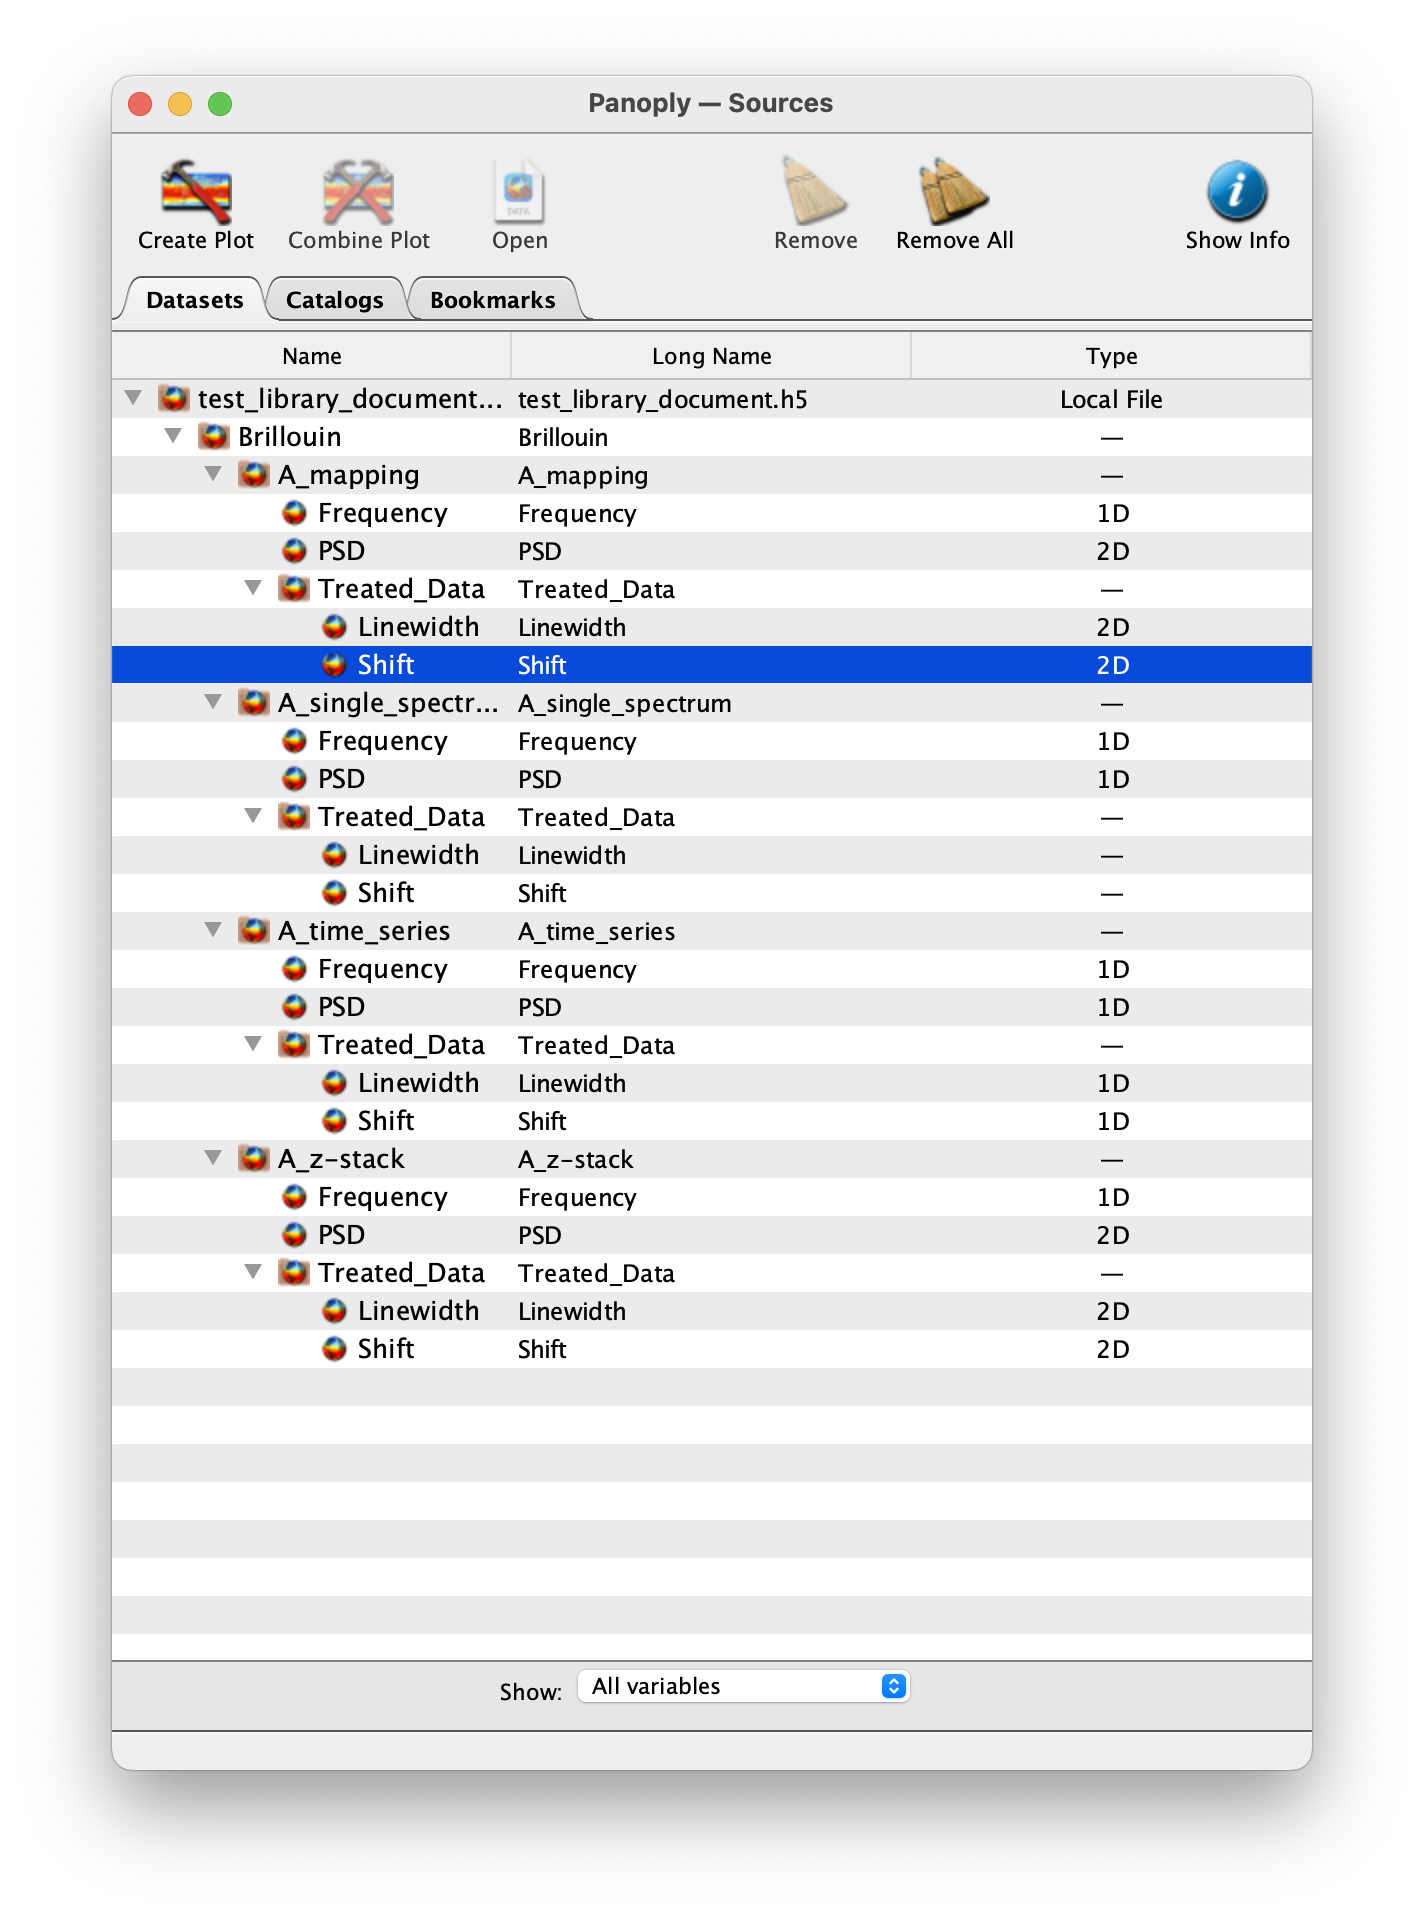
\includegraphics[width=0.4\textwidth]{img/Panoply_developed_structure.png}
    \caption{A simple visualization of the HDF5 file structure using the Panoply application} 
    \label{fig:panoply_developed_structure}
\end{figure}

\begin{figure}[H]
    \centering
    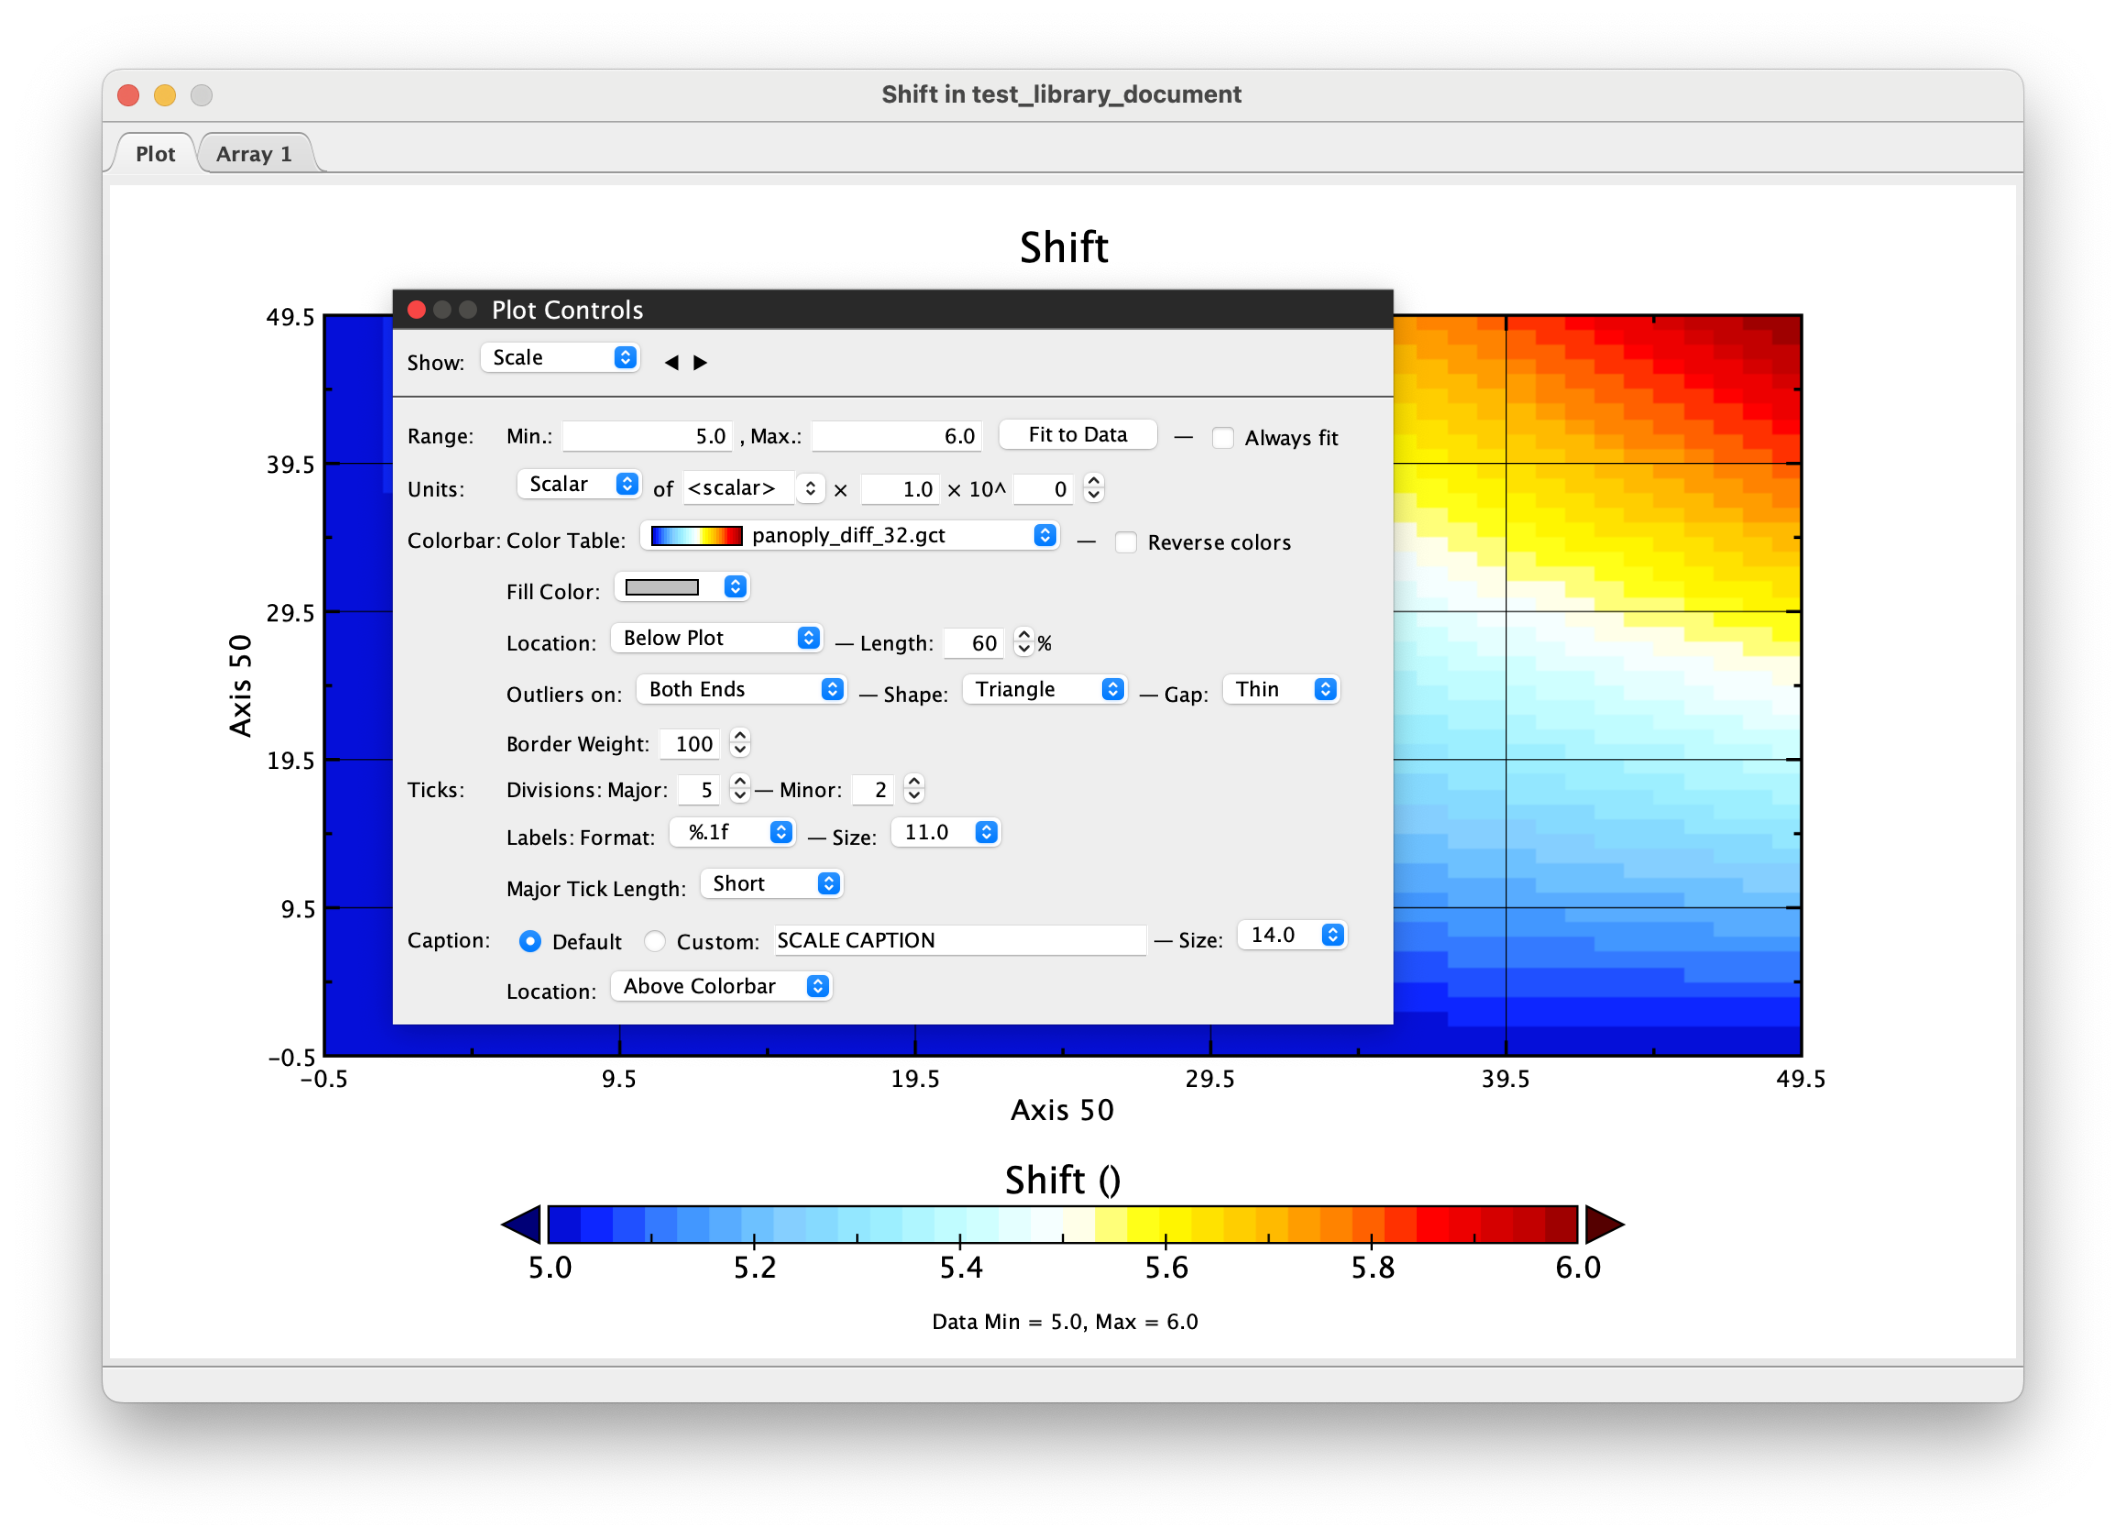
\includegraphics[width=0.7\textwidth]{img/Panoply_viewer.png}
    \caption{Visualizing datasets using the Panoply application} 
    \label{fig:panoply_viewer}
\end{figure}

\subsection{The HDF5\_BLS\_GUI}

The HDF5\_BLS\_GUI is a graphical user interface for the HDF5\_BLS package, designed to facilitate the exploration and analysis of HDF5 files. It provides a user-friendly environment for users to create and interact with their data. The GUI is meant to evolve to allow users to treat their data from it, but these developments are still in a beta phase. 

To use the GUI, you need to install the package. Follow the instructions below:

\begin{itemize}
    \item Clone the repository: \texttt{git clone https://github.com/yourusername/HDF5\_BLS.git}
    \item Navigate to the directory: \texttt{cd HDF5\_BLS}
    \item Install the packages for the GUI: \texttt{pip install -r requirements\_GUI.txt}
    \item Run the GUI: \texttt{python HDF5\_BLS\_GUI/main.py}
\end{itemize}

You should see the HDF5\_BLS\_GUI window appear on your screen (figure \ref{fig:gui_main_window}).

\begin{figure}[H]
    \centering
    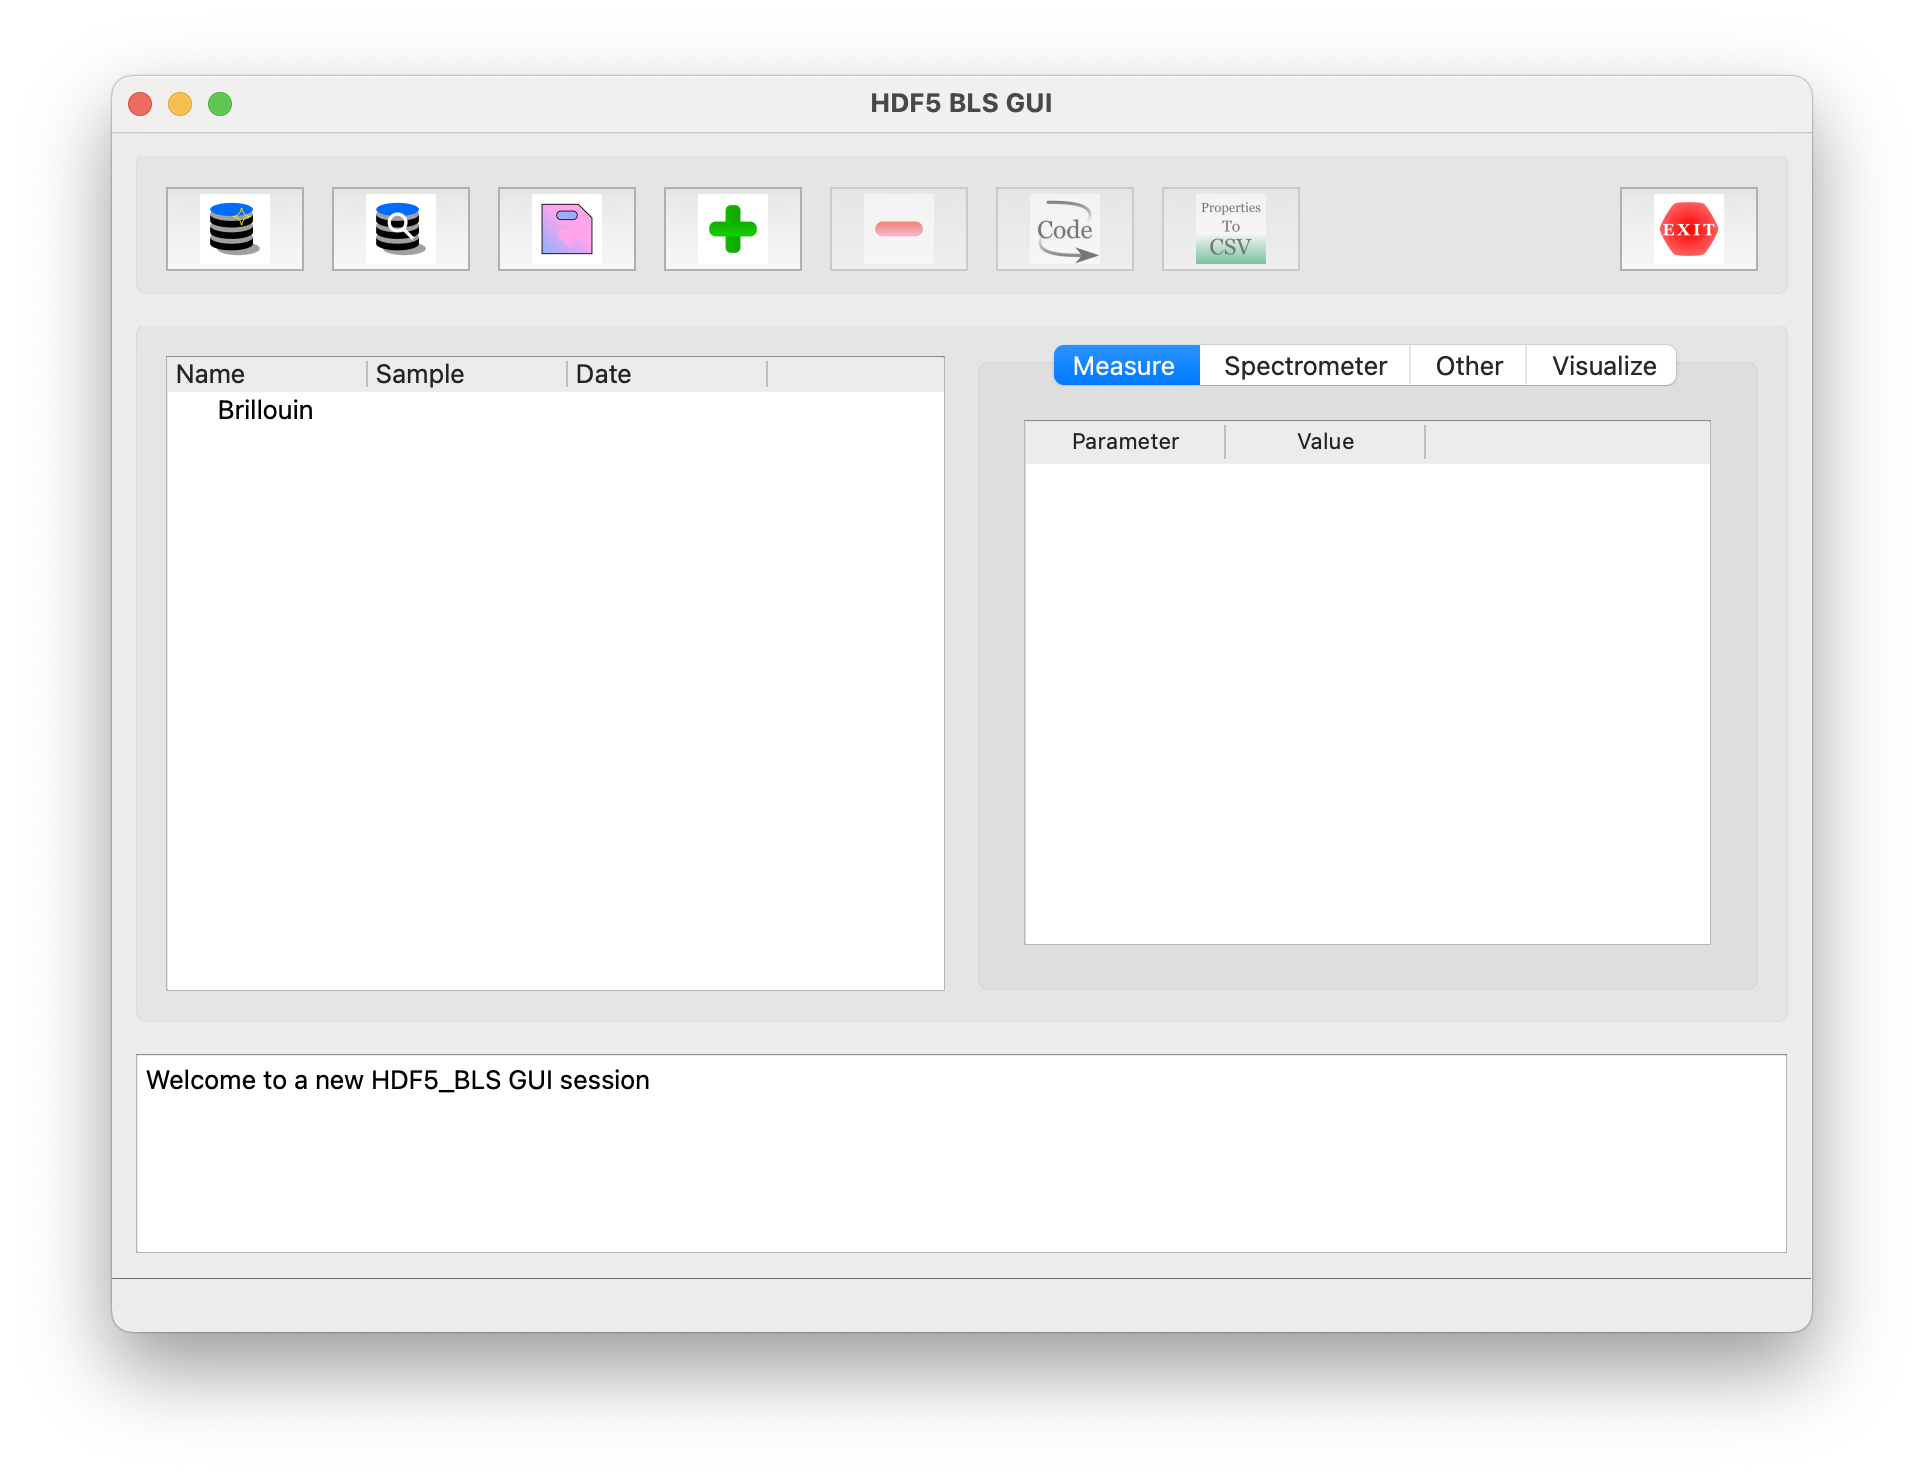
\includegraphics[width=0.8\textwidth]{img/HDF5_BLS_GUI_welcome.png}
    \caption{The welcome window of the HDF5\_BLS\_GUI}
    \label{fig:gui_main_window}
\end{figure}

You can then drag and drop your data into the left panel if its addition is already supported by the GUI. If not, you'll be forced to add it from script. 

You can then structure your file by creating groups, renaming them, dragging files from groups to groups, and generally use the GUI as you would a normal file explorer.

When adding a data, the GUI automatically creates a new group in the HDF5 file. You can change the name of the group by double clicking on it. You can also drag excel files with properties to the right panel to apply metadata to groups.

You can of course drag and drop the BrimX file we have created in this tutorial to the left panel to see its structure (figure \ref{fig:brimx_structure}).

\begin{figure}[H]
    \centering
    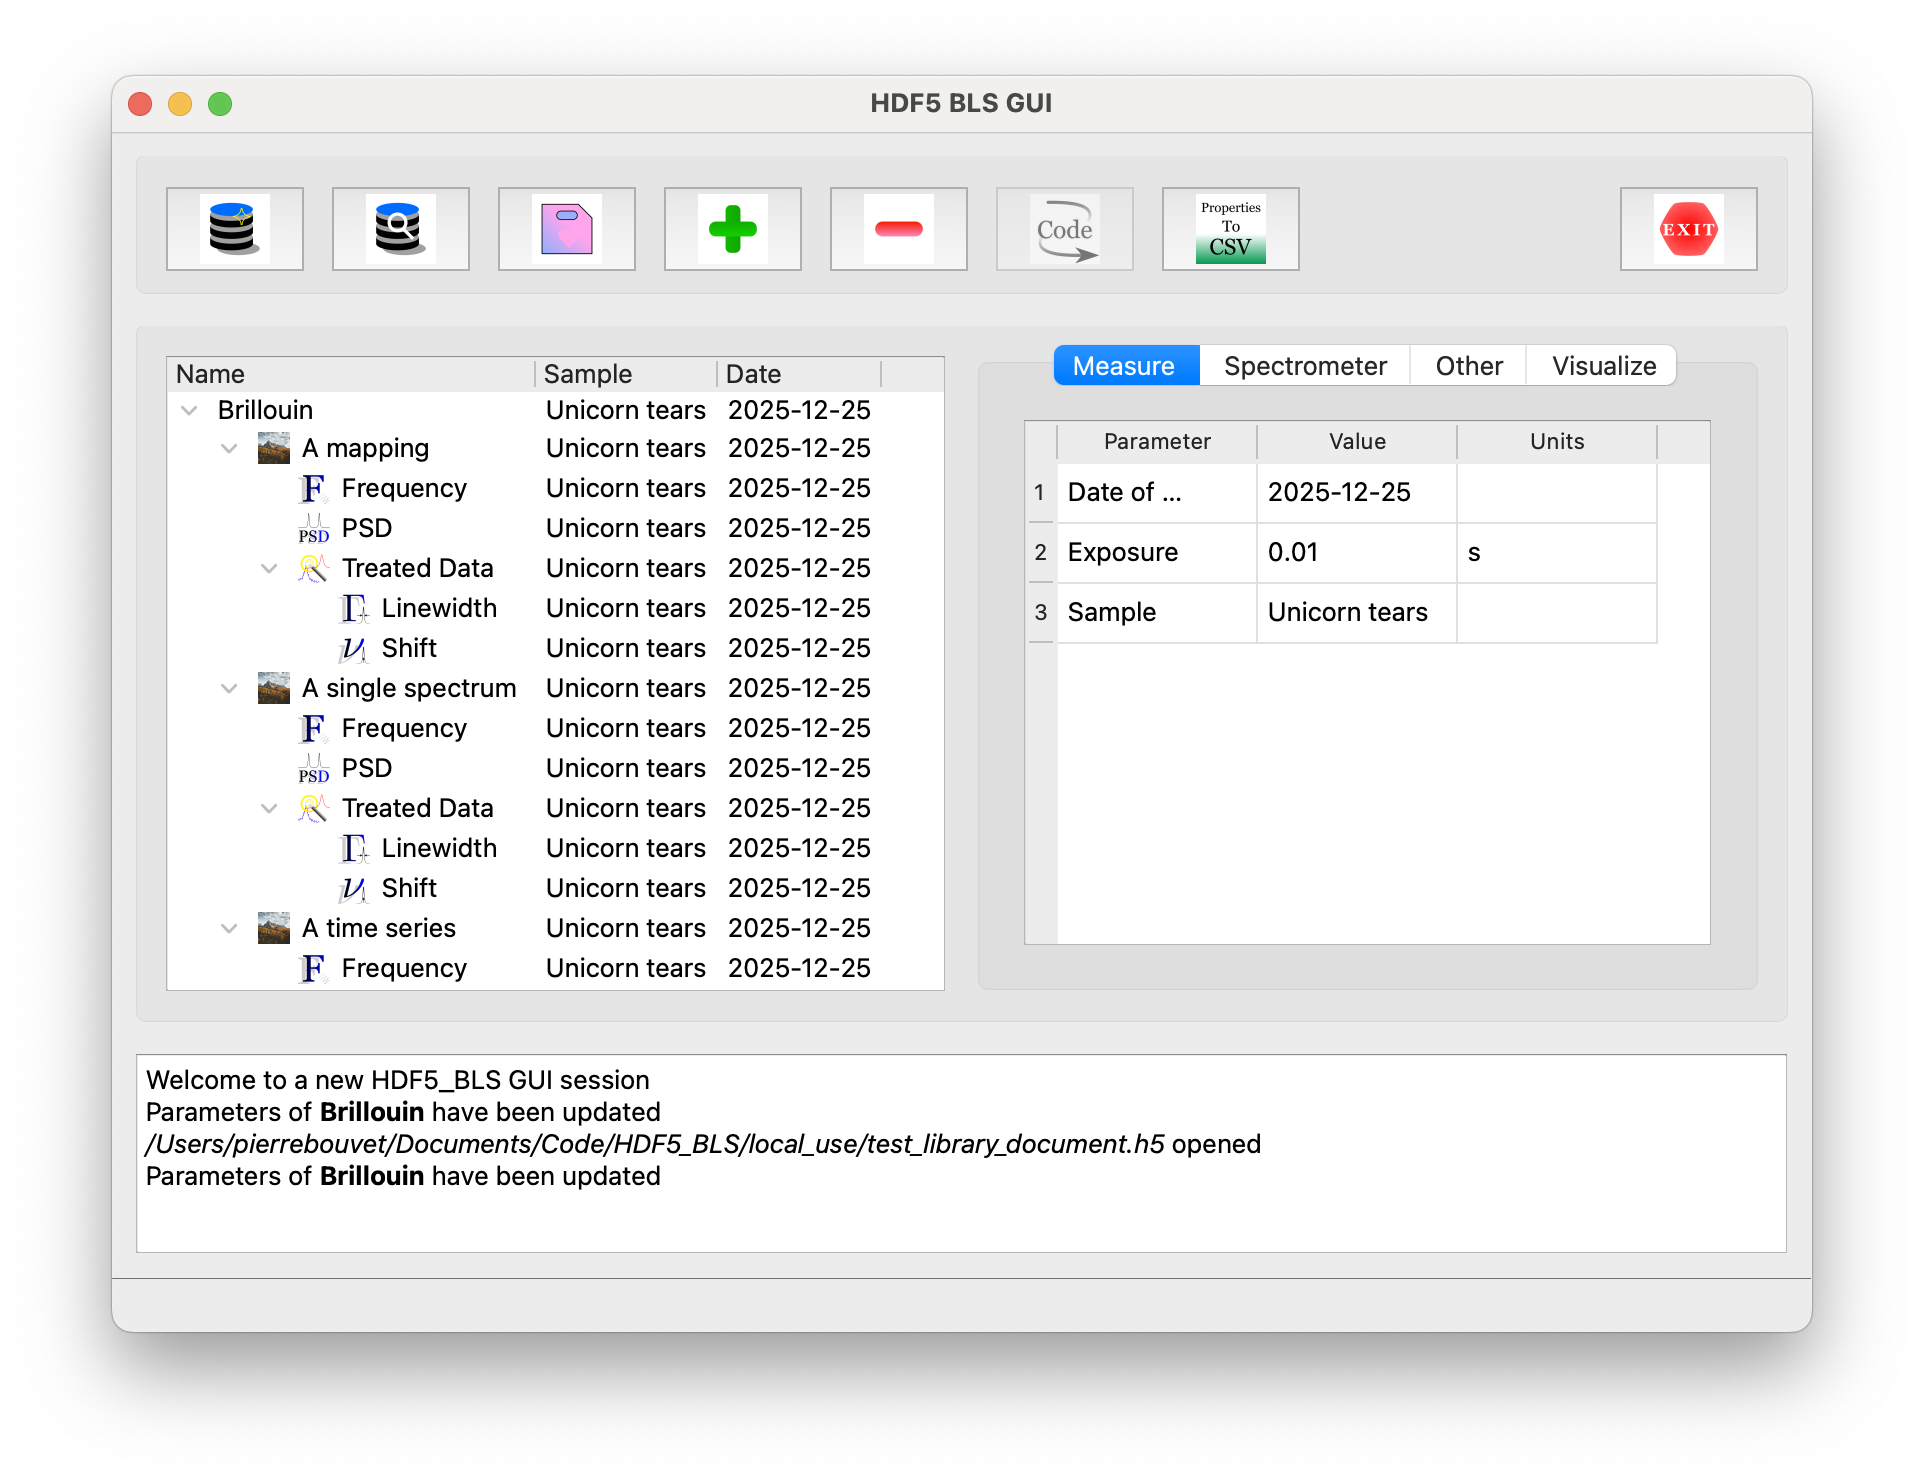
\includegraphics[width=0.8\textwidth]{img/HDF5_BLS_GUI_BrimX_structure.png}
    \caption{The structure of the example BrimX file in the HDF5\_BLS\_GUI}
    \label{fig:brimx_structure}
\end{figure}

This GUI is still in development, so don't hesitate to report bugs or suggest features on the GitHub repository: \url{https://github.com/bio-brillouin/HDF5_BLS/issues}.

\subsection{Ending remarks}

In this tutorial, we have covered the basics of using the HDF5\_BLS\_GUI for exploring and managing HDF5 files. We encourage you to experiment with the GUI and provide feedback to help us improve it. You can directly contact me at \href{mailto:pierre.bouvet@meduniwien.ac.at}{pierre.bouvet@meduniwien.ac.at} !

\vspace{5\baselineskip}

\section{HDF5\_BLS\_treat package}

The HDF5\_BLS\_treat package is a Python library designed to standardize the treatment and analysis of Brillouin data stored in HDF5 format. It provides a set of tools and functions to process Brillouin data and comes with a built-in recording tool to store the steps of the analysis for easy replication and storage.

\subsection{Installation}

We recommend setting up a virtual environment to install the package. This can be done using the following command:

\begin{tcolorbox}[colback=blue!5, colframe=blue!40!black, boxrule=0.5mm, sharp corners, left=2mm, right=2mm, top=1mm, bottom=1mm]
- On Mac terminal
\begin{lstlisting}
python -m venv HDF5_BLS_venv
source HDF5_BLS_venv/bin/activate 
\end{lstlisting}
\end{tcolorbox}

\begin{tcolorbox}[colback=yellow!5, colframe=yellow!40!black, boxrule=0.5mm, sharp corners, left=2mm, right=2mm, top=1mm, bottom=1mm]
- On Windows terminal
\begin{lstlisting}
python -m venv HDF5_BLS_venv
HDF5_BLS_venv\Scripts\activate
\end{lstlisting}
\end{tcolorbox}

On both OS, the package can be installed using pip:
\begin{lstlisting}
pip install HDF5_BLS_treat
\end{lstlisting}

\subsection{An example}

\subsubsection{Creating a synthetic spectrum}

Let's first create a synthetic spectrum, with a shift of 5GHz and a linewidth of 1GHz, an amplitude of 10 and an offset of 1:
\begin{lstlisting}
nu = np.linspace(-15, 15, 1024)
PSD = DHO(nu, 5, 1, 10, 1)
\end{lstlisting}


\subsubsection{Initialization}

The treatment will be performed on these two arrays. Let's thus initialize our treatment object:
\begin{lstlisting}
from HDF5_BLS_treat.treat import Treat
treat = Treat(frequency=nu, PSD=PSD)
\end{lstlisting}


\subsubsection{Normalization of the spectra}

A good practice is to normalize the data before applying the treatment. This can be done using the \texttt{normalize} function, after having defined one of multiple peaks to be considered as the norm (ie: the average of their amplitude is set to 1). To do so, we start by identifying the peaks to normalize. Here let's take only the Stokes peak. We select the peak by providing an approximation of its position (attribute "position\_center\_window") and a window size where to search for it  (attribute "window\_width"). We can also indicate the nature of this peak (attribute "type\_pnt" that can be set to "Stokes", "Anti-Stokes" or "Other"), although in this case, this doesn't matter much since we are averaging amplitudes regardless of the nature of the peak.
\begin{lstlisting}
treat.add_point(position_center_window = 5, type_pnt = "Other", window_width = 3)
\end{lstlisting}

Now we can normalize the data. This function identifies the noise level in the spectrum, averages it, substracts it from the data, and then divides the data by the average of the amplitude of all peaks that have been given with the "add\_point" function. To identify the noise level, we use the "threshold\_noise" attribute. This attribute defines the highest possible value of the noise level, given as a ratio of the difference of the maximum and minimum of the data. By default, this value is set to 1\%. Let's set it here to 5\%.
\begin{lstlisting}
treat.normalize(threshold_noise = 0.05)
\end{lstlisting}

\subsubsection{Identification of the points to fit}

Here we can start the fitting procedure. We first need to identify the peaks we want to fit. As before, we use the "add\_point" function to do so. In this case, we will fit the Stokes peak and the Anti-Stokes peak. Here it is important to indicate the nature of the peaks (attribute "type\_pnt" that can be set to "Stokes", "Anti-Stokes" or "Other") as we'll need to know that parameter to obtain a unique value of shift and linewidth to describe the spectrum.
\begin{lstlisting}
treat.add_point(position_center_window = -5, type_pnt = "Anti-Stokes", window_width = 3)
treat.add_point(position_center_window = 5, type_pnt = "Stokes", window_width = 3)
\end{lstlisting}

\subsubsection{Definition of the lineshape to use for the fit}

Different models are given to fit the data. You can for example decide to fit your peaks with a Lorentzian or a DHO lineshape. To tell the treatment which lineshape to use, you can use the "define\_model" function with the name of the model given in the "name" argument. You can also indicate if a line should also be fitted. This is a simple yet effective way to reduce the effect of a possible badly attenuated elastic peak. This is done by setting the "elastic\_correction" argument to True. Here let's use a DHO lineshape with no elastic correction:
\begin{lstlisting}
treat.define_model(name = "DHO", elastic_correction = False)
\end{lstlisting}

\subsubsection{Initial parameters}

A crucial step of any fitting procedure is the definition of the initial parameters. We have normalized the spectra so we have an initial guess for the amplitude of 1, and for the offset of 0. We have also defined the position of our peaks, so this value is also initialized. We haven't however defined the initial guess for the linewidth. The easiest way to estimate the width is to use the "estimate\_width\_inelastic\_peaks" function. Given the amplitude of the peak, this function takes the points of the curve that are approximately at the half height and deduces a value for the linewidth. To prevent aberrant values, we can provide a maximum value for the width (attribute "max\_width\_guess"). Here let's set it to 2GHz:

\begin{lstlisting}
treat.estimate_width_inelastic_peaks(max_width_guess = 2)
\end{lstlisting}

\subsubsection{Fitting the data}

Everything is setup now to fit the spectra. You can perform this fit one of two ways: either you fit each peak individually or fit all the peaks at once. To choose between the two methods, you can use the "single\_fit\_all\_inelastic" (fits every peak invidually) or the "multi\_fit\_all\_inelastic" (fits all the peaks at once) function. Both function have the same parameters:
\begin{itemize}
    \item "guess\_offset": a boolean that indicates whether the offset should be guessed or not. It might be interesting to force the offset to 0 if you know there's no offset in your data after normalization.
    \item "update\_point\_position": a boolean that indicates whether the position of the points should be updated during the fit. This is interesting if you're looping the fitting over a large number of spectra, as the position of the peak might change from one spectrum to another due to linear effects (temperature for example). 
    \item "bound\_shift": a tuple that defines the lower and upper bounds for the shift parameter.
    \item "bound\_linewidth": a tuple that defines the lower and upper bounds for the linewidth parameter.
\end{itemize}
To define the bounds for the shift and linewidth parameters, you can simply give a list (or tuple) of the lower and upper bounds for each fitted peak. For example, in this example, it would be weird to get values of shift lower than -5.5GHz and higher than -4.5GHz for the anti-Stokes peak, lower than 4.5GHz and higher than 5.5GHz for the Stokes peak, and linewidths lower than 0.9Ghz and higher than 1.1GHz. We can thus define the bounds and indicate the fitting as follows:

\begin{lstlisting}
bound_shift = [(-5.5, -4.5), (4.5, 5.5)]
bound_linewidth = [(0.9, 1.1), (0.9, 1.1)]
treat.multi_fit_all_inelastic(guess_offset=True, update_point_position=True, bound_shift= bound_shift, bound_linewidth=bound_linewidth)  
\end{lstlisting}

Note that at this step, an error on the value of the shift and linewidth is also obtained by estimating the Hessian matrix from the extrapolated Jacobian matrix.

\subsubsection{Applying the treatment to a multidimensional PSD dataset}

Up to here, we were working with a single spectrum. However, you'll often have a PSD dataset that stores multiple spectra. To apply the treatment to a multidimensional PSD dataset, you can use the "apply\_algorithm\_on\_all" function. This function takes no arguments, it simply runs all the steps sequentially on each spectrum of the dataset, considering that the last dimension is the one of the channels.

\begin{lstlisting}
treat.apply_algorithm_on_all()
\end{lstlisting}

\subsubsection{Combining fits}

In most cases, you'll want to combine the results of fits performed on a series of peaks. Under the hypothesis of symmetry, you can do that using the "combine\_results\_FSR" function. This function considers the type of the peaks, and given a FSR (Free Spectral Range), for the spectrometer, it combines the results of the fits of the peaks. If order N is centered on the 0 of the frequency axis, then it will automatically subtract to the shift of the peaks of order N+1 and N-1 the corresponding FSR offset to get a shift value contained in [-FSR/2, FSR/2]. The function then extracts a single value for the shift and linewidth of all the peaks. It can do so by either considering only the peak of highest amplitude (attribute "keep\_max\_amplitude" set to True), by averaging the values of all the peaks weighing them by their amplitude (attribute "amplitude\_weight" set to True), by averaging the values of all the peaks weighing them by the error on the shift (attribute "shift\_err\_weight" set to True), or by simply averaging the values of all the peaks (all attributes set to False). Here let's consider a spectrometer with a FSR of 15GHz, and let's combine the results by weighing them by their error on the shift:

\begin{lstlisting}
treat.combine_results_FSR(FSR = 15, keep_max_amplitude = False, amplitude_weight = False, shift_err_weight= True)
\end{lstlisting}

\subsubsection{Getting the results}

Your fit is over! You can now get the results of the treatment. These are stored in the attributes of the "treat" object. The main attributes are:
\begin{itemize}
    \item "shift" -> where the shift is stored
    \item "linewidth" -> where the linewidth is stored
    \item "amplitude" -> where the amplitude is stored
    \item "offset" -> where the offset is stored
    \item "shift\_var" -> where the variance on the fitted shift is stored
    \item "linewidth\_var" -> where the variance on the fitted linewidth is stored
    \item "amplitude\_var" -> where the variance on the fitted amplitude is stored
\end{itemize}

\begin{lstlisting}
shift = treat.shift
linewidth = treat.linewidth
amplitude = treat.amplitude
\end{lstlisting}

\subsection{A code to try}

If you don't want to read the last section, you can directly try the following code:

\begin{lstlisting}

from HDF5_BLS_treat.treat import Treat, Models
import sys

nu=np.linspace(-15, 15, 1024)
gradient_x=np.linspace(0, 1, 50)
gradient_y=np.linspace(0, 1, 50)
temp=(np.outer(gradient_y, gradient_x) + np.outer(gradient_y, gradient_x))/2
shift_2D=temp + 5
linewidth_2D=temp + 1 
PSD_2D=np.zeros((50, 50, 1024))
for i in range(50):
    for j in range(50):
        PSD_2D[i, j]=DHO(nu, shift_2D[i, j], linewidth_2D[i, j], 1, 0) 

treat=Treat(frequency=nu, PSD=PSD_2D)

treat.add_point(position_center_window=5.5, type_pnt="Stokes", window_width=1)
treat.normalize_data(threshold_noise=0.05)

treat.add_point(position_center_window=-5, type_pnt="Anti-Stokes", window_width=3)
treat.add_point(position_center_window=5, type_pnt="Stokes", window_width=3)

treat.define_model(model="DHO", elastic_correction=False)

treat.estimate_width_inelastic_peaks(max_width_guess=1)

bound_shift=[(-6.5, -4.5), (4.5, 6.5)]
bound_linewidth=[(0.9, 2.1), (0.9, 2.1)]
treat.multi_fit_all_inelastic(guess_offset=True, update_point_position=True, bound_shift= bound_shift, bound_linewidth=bound_linewidth)  

treat.apply_algorithm_on_all()
treat.combine_results_FSR(FSR=15, keep_max_amplitude=False, amplitude_weight=False, shift_err_weight= True)

plt.figure()
plt.subplot(131)
plt.imshow(treat.shift)
plt.title('Brillouin Shift (GHz)')
plt.colorbar()

plt.subplot(132)
plt.imshow(treat.linewidth)
plt.title('Line Width (GHz)')
plt.colorbar()

plt.subplot(133)
plt.imshow(treat.amplitude)
plt.title('Amplitude (a.u.)')
plt.colorbar()

plt.tight_layout()
plt.show()
\end{lstlisting}

\begin{center}
\textbf{Thank you for your help! Happy Brillouin data handling!}
\end{center}

\end{document}